\documentclass[12pt,titlepage]{article}
\usepackage[table]{xcolor}
\usepackage{longtable}
\usepackage[utf8]{inputenc}
%Language of Document Elements like Figure or Table
\usepackage[english]{babel}
\usepackage[bookmarks]{hyperref}
\usepackage{pdfpages}
\usepackage{graphicx}
\usepackage{float}
\usepackage{array}
\usepackage{lipsum} 
\usepackage[justification=centering]{caption}
\usepackage{enumitem}
\usepackage{chngcntr}
\usepackage{lscape}
\usepackage{fancyhdr}
\usepackage{listings}
\usepackage[style=alphabetic, backend=biber]{biblatex}
\usepackage{dafny}
\usepackage{hyperref}
\usepackage{nameref}
\usepackage[margin=1in]{geometry}

%Each Section in a new Page
\let\oldsection\section
\renewcommand\section{\clearpage\oldsection}

%Set space around and between lists
\setlist[enumerate]{noitemsep, topsep=0cm}
\setlist[itemize]{noitemsep, topsep=0cm}

%Figure/Table Numbering style "Section Number.figure counter
\renewcommand{\thefigure}{\arabic{section}.\arabic{figure}}
\renewcommand{\thetable}{\arabic{section}.\arabic{table}}

%Reset figure/table counter after section change
\counterwithin{figure}{section}
\counterwithin{table}{section}

%Syntax Highlighting
%\lstdefinestyle{dafny}{
%	language=dafny, 
%	basicstyle=\normalfont\ttfamily,
%	numbers=left,
%	numberstyle=\scriptsize,
%	stepnumber=1,
%	numbersep=8pt,
%	showstringspaces=false,
%	breaklines=true,
%	frame=lines,
%	backgroundcolor=\color{background}
%}

\colorlet{punct}{red!60!black}
\definecolor{background}{HTML}{EEEEEE}
\definecolor{delim}{RGB}{20,105,176}
\colorlet{numb}{magenta!60!black}

\lstdefinelanguage{json}{
	basicstyle=\normalfont\ttfamily,
	numbers=left,
	numberstyle=\scriptsize,
	stepnumber=1,
	numbersep=8pt,
	showstringspaces=false,
	breaklines=true,
	frame=lines,
	backgroundcolor=\color{background},
	literate=
	*{0}{{{\color{numb}0}}}{1}
	{1}{{{\color{numb}1}}}{1}
	{2}{{{\color{numb}2}}}{1}
	{3}{{{\color{numb}3}}}{1}
	{4}{{{\color{numb}4}}}{1}
	{5}{{{\color{numb}5}}}{1}
	{6}{{{\color{numb}6}}}{1}
	{7}{{{\color{numb}7}}}{1}
	{8}{{{\color{numb}8}}}{1}
	{9}{{{\color{numb}9}}}{1}
	{:}{{{\color{punct}{:}}}}{1}
	{,}{{{\color{punct}{,}}}}{1}
	{\{}{{{\color{delim}{\{}}}}{1}
	{\}}{{{\color{delim}{\}}}}}{1}
	{[}{{{\color{delim}{[}}}}{1}
	{]}{{{\color{delim}{]}}}}{1},
}


%TODO
\newcommand{\todonl}[1]{\newline\textcolor{red}{TODO: #1}\PackageWarning{TODO:}{#1!}}
\newcommand{\todo}[1]{\textcolor{red}{TODO: #1}\PackageWarning{TODO:}{#1!}}

%Set Paragraph indent to null
\setlength{\parindent}{0pt}
% Smaler Table Space
\renewcommand{\arraystretch}{1.5}

\title{Visual Studio Code Integration for the Dafny Language and Program Verifier}
\author{Rafael Krucker, Markus Schaden}
\date{20.02.2017}

\pagestyle{fancy}
\lhead{BA Dafny}
\addbibresource{LITERATURVERZEICHNIS/bibliographie.bib}
\begin{document}
\pagenumbering{Roman} 

% TODO
%
\includepdf{titlepage/titlepage}

% TODO
%\phantomsection
\addcontentsline{toc}{section}{Abstract}
\section*{Abstract}
[Placeholder Abstract Text]
%\newpage
%\phantomsection
\addcontentsline{toc}{section}{Management Summary}
\section*{Management Summary}
\subsection*{Ausgangslage}
[Placeholder]

\subsection*{Vorgehen}
[Placeholder]

\subsection*{Technologien}
[Placeholder]

\subsection*{Ergebnisse}
[Placeholder]

\subsection*{Ausblick}
[Placeholder]


% TODO
%\includepdf[pages={1-}, 
%scale=0.9,pagecommand=\thispagestyle{plain}]{additionals/eigenstaendigkeit}
%\includepdf[pages={1-2}, 
%scale=0.9,pagecommand=\thispagestyle{plain}]{additionals/aufgabenstellung}

\newpage
\tableofcontents
\newpage
\pagenumbering{arabic}
\section{Abstract}
The goal of this project is to integrate the Dafny programming language into Visual Studio Code. Emphasis is put into researching how Dafny programmers can be best supported during their work and how writing code can be made more productive. \newline

Since Dafny offers built-in specification constructs, novel work is to provide tooling that makes working with them easier. The most beneficial feature would be to implement a generic, context aware proof obligation generator that continuously suggests specification constructs to the programmer. This approach was eventually discarded because it was deemed to hard to make it work with the proof engine that Dafny uses. Instead, situations were identified that arise often during programming and specific aid with specification constructs was implemented for those situations. Another helpful Dafny specific features is the displaying of counter examples where the code written does not satisfy the corresponding specification constructs, allowing quick discovery of edge cases and refinement of specification constructs. \newline

Next to language specific features, standard IDE mechanisms allow for great improvement regarding productivity. It was therefore deemed paramount that the project implements the most common features such as go to definition, renaming refactorings and find references. This was achieved using the standard interfaces that Visual Studio Code provides for these use cases, allowing programmers accessing these features in a well established way. \newline

Regarding the fact that Dafny is still a very young language, it is an important concern that new users can get started quickly, so that the user base continuous to grow. To support this, automatic installation of the plugin on all major platforms was implemented. Next to the plugin itself, the installation also resolves all dependencies such as the Dafny compiler itself. To further maximize portability, the plugin implements the language server protocol. This allows for writing IDE agnostic language analysis platforms, making the plugin not only usable in Visual Studio Code, but also integrable into other IDEs such as Emacs with only minor adjustments. \newline

This project concluded with the implementation of a production ready integration of Dafny into Visual Studio Code. The application of continuous integration allowed for a user base of about 300 people at the end of this writing, proofing that the plugin is robust and works across multiple environments. Dafny programmers are supported in their coding not only with standard IDE mechanisms, but also Dafny specific features. This not only makes the experience of programming more productive, but lays the foundation of a contentiously growing Dafny community. \newline

\section{Management Summary}
Following the quickly growing digitalization of businesses and the therefore more complex applications being developed, two key points are gaining focus in today's IT landscape. The first one is the proven functional correctness of programs and the second one is the uprising of multi threaded applications. Writing multi threaded applications becomes much simples once the functional correctness is proven, thus it can be stated that proven functional correctness is a stepping stone towards the easier implementation of parallelism. Dafny is a programming language which tries to move the focus of writing correct code towards writing correct specification constructs, which is often easier. Applying this concept consistently should result in being able to turn business requirements into correct working implementations quicker as with traditional languages. The proven correlation between the time of discovering an error and the cost of fixing it also strongly advises writing software which is proven correctly as early in the life cycle of the product as possible. Even though using Dafny in business is compelling for these reasons, its usage is still not widespread, something which this project tries to change.\newline

The wide spread usage of a tool for programmers is mainly dictated by two factors, namely the burden of getting it to run and the support that it is able to offer the programmer. \newline

To address the first point, the plugin was developed for Visual Studio Code, an IDE running on all major platforms. It was also given an installation routine which resolves all dependencies on all platforms automatically after pressing one button. This also allows programmers that are not that familiar with the console to rapidly develop Dafny programs, something that was not possible given the tooling existing up until now. \newline

Regarding the second point, it was always paramount to offer as much help as possible to the programmer. This was done in two steps, the first one being implementing standard features that a programmer is used to when working with an IDE, which could be achieved within this project. The second step are language specific features. To offer these, some research was done in what situations often arise when programming Dafny in order to reveal which features a programmer could most benefit from without solving all specification construct suggestions in a generic way. This pragmatic approach helped the project stay in scope while still offering rich help in many common programming contexts. \newline

While at first not a key concern, it was decided to implement the plugin according to an emerging standard in semantic language analysis platforms. This means that the plugin does not only work well with Visual Studio Code, but can be integrated into many other IDEs such as Emacs with very little adjustments, further broadening the possible Dafny user base. \newline

During the project, production quality was always striven for, so that the end product was not a prototype which no one uses. Due to the application of continuous integration the user base of the plugin has already reached 300 people at the time of this writing, proving the usability and robustness of the product developed by this project. The project remains open source, inviting other to continue the work and share the benefits of Dafny with even more people. \newline
\section{Outline}
\subsection{The problem and its setting}
This chapter presents the background of the project, the problem and its significance.
\subsubsection{Introduction}
Dafny is a language designed and implemented by Microsoft Research. It offers built-in specification constructs. These include pre- and postconditions, frame specifications as well as termination metrics. Further support such as ghost variables and recursive functions are also implemented. Through such specification primitives, the Dafny verifier, invoked during compilation, can be used to verify the specified aspects of the functional correctness of the program. \newline
Dafny is typically used via its Visual Studio IDE integration under the Windows operating system. This allows for an efficient work flow of editing a program while constantly being given feedback about its functional correctness. The Dafny compiler and verifier can additionally be invoked from the command line. \newline
Microsoft would like to integrate of Dafny into the cross-platform Visual Studio Code IDE. Work on this has already been started through a plugin by Jonathan  Rionatan. It currently works within the mono-environment and provides feedback from the verifier. \newline

\subsubsection{Statement of the problem}
This thesis aims to research on how Dafny programmers can be best supported during their work and incorporate these findings in a production quality plugin for Visual Studio Code. 
\subsubsection{Significance of study}
Standard programming techniques are beginning to show their limitations as multi-core and multi-threaded applications are becoming more and more popular, which are difficult and error prone.
Proving functional correctness has the potential of helping the programmer construct reliable programs.
Sadly, the use of this technology is not yet widespread. Providing better tool support has the potential of improving this situation. Here lies the significance of this project.
\subsubsection{Scope and delimitation}
The plugin is limited to be used in three defined environments, although they compromise a huge percentage of environments used in programming. The plugin offers a fixed set of features which are detailed in this thesis, but remains open for adaption and extension.
\subsubsection{Definition of terms}

\section{Use Cases}
\subsection{Use Case Diagram}
\begin{figure}[h]
	\centering
	\includegraphics[width=1\linewidth, height=5in]{"./img/UseCase"}
	\caption{Use Case Diagram}
	\label{fig:usecase-diagram}
\end{figure}
\subsection{Actors and Stakeholder}
\begin{itemize}
	\item Programmers
	\item Microsoft
\end{itemize}
\subsection{Descriptions (brief)}
\subsubsection{UC1: Easy installation of Dafny plugin}
A programmer can simply install the Dafny plugin by running an automatic installer which sets all path variables and makes additional needed environment adjustments. This can be done on Windows 10 in a .NET environment or either on Linux or OSX in a mono environment.
\subsubsection{UC2: Syntax Highlighting}
The system automatically does syntax highlighting while the user writes a Dafny (dfy.) file.
\subsubsection{UC3: Reporting of Dafny best practices violations}
The plugin can be configured with a simple DSL config file which describes common best practices for Dafny. The plugin reports violations of these rules via the standard Visual Studio Code notification mechanisms.
\subsubsection{UC4: Automatic generation of contracts}
The plugin can be configured with a simple DSL-File to recognize certain situations, which could benefit from the setting of pre- and postconditions. The plugin offers to add these in form of a refactoring via the common Visual Studio Code mechanisms.

\subsubsection{UC5: Autocompletion for identifiers}
The plugin offers autocompletion of Dafny code while the user types via the standard Visual Studio Code mechanisms.
\subsection{Descriptions (fully dressed)}

\subsubsection{UC1: Easy installation of Dafny plugin}
\rowcolors{1}{gray!25}{white}
\begin{longtable}{l | p{0.7\textwidth} }
	Description & A programmer can simply install the Dafny plugin by running an automatic installer which sets all path variables and makes additional needed environment adjustments.\\ \hline
	Primary Actor & Programmer\\ \hline
	Trigger & Programmer wants to install the Dafny plugin to Visual Studio Code.\\ \hline
	Stakeholder and Interests & Programmer: Wants an easy, automated installation of the plugin. \newline Microsoft: Wants a stable Dafny integration to fulfill the needs of its clients.\\ \hline
	Preconditions &\begin{itemize}
		\item Depending on the environment, either the .NET or the mono framework are installed.
		\item Visual Studio Code is installed.
		\item The programmer has admin privileges in his environment.
	\end{itemize}\\ \hline
	Postconditions & 
	\begin{itemize}
		\item The plugin works without problems, the programmer can start writing code.
	\end{itemize} \\ \hline
	Main Success Scenario & 
	1. Programmer downloads the plugin via the Visual Studio Code plugin store. \newline
	2. The plugin determines which platform it is run on, and sets either the path to the .Net framework or the mono framework. \newline
	3. The plugin downloads Dafny and sets the path to the DafnyServer binary. \newline
	4. The plugin then installs itself via the standard Visual Studio Code plugin mechanisms. \newline
	5. The plugin prompts a success message and the programmer is ready to code in Dafny.\\ \hline
	Extensions & 
	2a. The installer cannot find, depending on the environment, either the mono or the .Net framework in the standard locations. \newline 
	- It prompts the user to enter the location and does so until the framework is found. \\ \hline
	Special Requirements & None\\ \hline
	Frequency of Occurrence & Usually once per working environment\\ \hline
	Open Issues & None \\ \hline
	\caption{UC1}
\end{longtable}

\subsubsection{UC2: Syntax Highlighting}
\begin{longtable}{l | p{0.7\textwidth} }
	Description & The system automatically does syntax highlighting while the user writes a Dafny (.dfy) file.\\ \hline
	Primary Actor & Programmer\\ \hline
	Trigger & Programmer writes Dafny code in Visual Studio Code.\\ \hline
	Stakeholder and Interests & Programmer: Wants enhanced readability for the source files he is working on. \newline Microsoft: Wants a state of the art IDE integration of Dafny.\\ \hline
	Preconditions &
	\begin{itemize}
		\item Visual Studio Code with the Dafny plugin installed is running.
		\item Dafny code is being written in a .dfy file.
	\end{itemize}\\ \hline
	Postconditions &
	\begin{itemize}
		\item The source code is highlighted in different colors according to common standards in general and the Visual Studio Code guidelines specifically.
	\end{itemize}\\ \hline
	Main Success Scenario & 
	1. Programmer types code into a .dfy file. \newline
	2. The plugin detects the changes and applies syntax highlighting through the standard Visual Studio Code mechanisms.\\ \hline
	Extensions & 
	2a. The newly written code causes a compilation error and cannot be interpreted. \newline 
	- The previous syntax highlighting stays in place, the errors are highlighted according to common practices with compilation errors in Visual Studio Code. \\ \hline
	Special Requirements & None\\ \hline
	Frequency of Occurrence & Very often, after every key up event.\\ \hline
	Open Issues & None \\ \hline
	\caption{UC2}
\end{longtable}

\subsubsection{UC3: Reporting of Dafny best practices violations}
\begin{longtable}{l | p{0.7\textwidth} }
	Description & The plugin can be configured with a simple DSL config file which describes common best practices for Dafny. The Plugin reports violations of these rules via the standard Visual Studio Code notification mechanisms.\\ \hline
	Primary Actor & Programmer\\ \hline
	Trigger & Programmer writes Dafny code in Visual Studio Code.\\ \hline
	Stakeholder and Interests & Programmer: Wants to write the cleanest code possible using common Dafny idioms. \newline Microsoft: Wants to support programmers getting the most out of Dafny.\\ \hline
	Preconditions &
	\begin{itemize}
		\item Visual Studio Code with the Dafny plugin installed is running.
		\item Dafny code is being written in a .dfy file.
	\end{itemize}\\ \hline
	Postconditions &
	\begin{itemize}
		\item Violations of common best practices for Dafny are reported through the standard Visual Studio Code mechanisms.
	\end{itemize}\\ \hline
	Main Success Scenario & 
	1. The plugin is installed preconfigured with a collection of common best practices for Dafny, which is done through a DSL file. \newline
	2. Programmer types code into a .dfy file. \newline 
	3. The plugin continuously checks for violations of the rules. \newline 
	4. If a violation is detected, it is reported through the standard mechanisms of Visual Studio Code.\\ \hline
	Extensions & 
	1a. The predefined rules are not sufficient for the programmer. \newline 
	- The programmer can update the configuration file himself to include his own or his company's coding guidelines. \\ \hline
	Special Requirements & None\\ \hline
	Frequency of Occurrence & Very often, after new valid syntax was written.\\ \hline
	Open Issues & None \\ \hline
	\caption{UC3}
\end{longtable}

\subsubsection{UC4: Automatic generation of contracts}
\begin{longtable}{l | p{0.7\textwidth} }
	Description & The plugin can be configured with a simple DSL-File to recognize certain situations which could benefit from the setting of pre- and postconditions. The plugin offers to add these in form of a refactoring via the common Visual Studio Code mechanisms.\\ \hline
	Primary Actor & Programmer\\ \hline
	Trigger & Programmer writes Dafny code in Visual Studio Code.\\ \hline
	Stakeholder and Interests & Programmer: Wants help to find appropriate contracts. \newline Microsoft: Wants to support programmers getting the most out of Dafny.\\ \hline
	Preconditions &
	\begin{itemize}
		\item Visual Studio Code with the Dafny plugin installed is running.
		\item Dafny code is being written in a .dfy file.
	\end{itemize}\\ \hline
	Postconditions &
	\begin{itemize}
		\item Specification constructs suitable for the context were added to the code.
	\end{itemize}\\ \hline
	Main Success Scenario & 
	1. The plugin is installed preconfigured with a collection of common situations for Dafny and their corresponding specification constraints, which is done through a DSL file. \newline
	2. Programmer types code into a .dfy file. \newline 
	3. The plugin continuously checks for situations that could benefit form the setting of specification constraints. \newline 
	4. If such a semantic is detected, it is reported through the standard mechanisms of Visual Studio Code, with a command offered to add the constraints. \newline
	5. The programmer invokes the refactoring and the necessary code is added.\\ \hline
	Extensions & 
	1a. The predefined situations and contract code additions are not sufficient for the programmer. \newline 
	- The programmer can update the configuration file himself to include support for his own or his company's  common code semantics. \\ \hline
	Special Requirements & None\\ \hline
	Frequency of Occurrence & Very often, upon typing code with no syntax errors.\\ \hline
	Open Issues & None \\ \hline
	\caption{UC4}
\end{longtable}

\subsubsection{UC5: Autocompletion for identifiers}
\begin{longtable}{l | p{0.7\textwidth} }
	Description & The plugin offers autocompletion of Dafny code while the user types via the standard Visual Studio Code mechanisms.\\ \hline
	Primary Actor & Programmer\\ \hline
	Trigger & Programmer writes Dafny code in Visual Studio Code.\\ \hline
	Stakeholder and Interests & Programmer: Wants to be more productive while writing Dafny code. \newline Microsoft: Wants a state of the art IDE integration of Dafny.\\ \hline
	Preconditions &
	\begin{itemize}
		\item Visual Studio Code with the Dafny plugin installed is running.
		\item Dafny code is being written in a .dfy file.
	\end{itemize}\\ \hline
	Postconditions &
	\begin{itemize}
		\item An identifier was autocompleted.
	\end{itemize}\\ \hline
	Main Success Scenario & 
	1. Programmer types code into a .dfy file. \newline
	2. The plugin detects the changes and searches for the beginning of known identifiers. \newline
	3. If such a beginning is found, completion if offered through the standard mechanisms of Visual Studio Code.\\ \hline
	Extensions & 
	None. \\ \hline
	Special Requirements & None\\ \hline
	Frequency of Occurrence & Very often, after every key up event.\\ \hline
	Open Issues & None \\ \hline
	\caption{UC5}
\end{longtable}
\section{Project management}
\subsection{Projectplan}
\begin{figure}[H]
	\centering
	\includegraphics[width=1\textwidth]{img/projectplan}
	\caption{Projectplan}
	\label{fig:Projectplan}
\end{figure}
\subsection{Milestones}
\rowcolors{1}{gray!25}{white}
\begin{longtable}[H]
	{l| l | l | p {0.6\textwidth}}
	\textbf{Nr} &\textbf{Date}  &\textbf{Title} & \textbf{Description} \\ 
	\hline\hline
	
	M1 & 26.03.2017 & First prototype & Plugin is working on all operation systems, simple verification is in place and errors are reported, basic syntax highlighting, automatic downloading of dependencies and installation of Dafny and configure of environment variables\\ 
	
	M2 & 30.04.2017 & Contract generation & First automatic contract generation, customizable with DSL \\ 
	
	M3 & 21.05.2017 & IDE features & Autocompletion for identifiers, adding support for common refactorings like renaming \\ 
	
	M4 & 04.06.2017 & Release 1.0 & Everything implemented and tested. Ready to be published \\ 		
	\caption{Milestone}
	\label{tab:Milestone}
\end{longtable}

\subsection{Risk management}
\begin{landscape}
	\rowcolors{2}{gray!25}{white}
	\begin{longtable}[H]
		{l|p{0.22\textwidth}| p{0.22\textwidth} | p{0.1\textwidth} | p{0.1\textwidth} | p{0.25\textwidth} | p{0.25\textwidth}}
		
		\textbf{Nr} & \textbf{Title} & \textbf{Description} & 
		\textbf{Max Harm [h]} & \textbf{Proba- bility} & \textbf{Prevention} &  
		\textbf{Behaviour at entry}\\ \hline
		
		R1 & Underestimation of workload & One or more team members cannot finish a feature in time or loses to much time on a minor feature & 70 & 25\% & Weekly scrum meetings with feedback about the current work progress. Estimate workload together. Include time reserve & Help each other, if one is struggling. Feature reduction as last resort. \\ 
		
		R2 & Workflow is not working & Toolchain is not working as planed. The used components are not ideal for the problem & 30 & 15\% & Use experience to get a good setup and test it alot in the beginning & Redefine toolchain or change single tool \\ 
		
		R3 & Communication problems & Team is not working together and each member is developing individually. Creation of incompatible interfaces. Talking with the industrial partner is not possible as expected, due to time difference or not enough time & 70 & 20\% & Weekly scrum meetings and agreements. Already worked in other projects as a team before & Increase written documentation and working closer together. Having a fixed meeting with the industrial partner \\ 
		
		R4 & Lack of knowledge & Team has to little knowledge about Dafny, VSCode and the development of a VSCode Plugin & 80 & 10\% & Already experience with typescript for plugin development, as preparatory work informed about Dafny & Find necessary knowledge online, get help from Microsoft Research \\ 
		
		R5 & Data loss or manipulation & Data loss because of a server crash or open permissions to access and modify data & 20 & 3\% & Regularly backups and restrictive permissions to change files & Use backup to restore data. Extend safety measures \\ 
		
		R6 & Failure developer machine & One of the developer machines is not working anymore. & 10 & 1\% & Limited, regularly commits and backups. & Switch temporary to the school computer and install the necessary tools. \\
		
		R7 & Implementing the DSL is too complicated or too difficult to use & The DSL would be needed to suggest possible contracts or to customize the best practices. & 100 & 30\% & This core feature has to be researched carefully so that it really fits our needs and that other developers can really use the plugin. & Read about DSL, talking to people which have already worked with it. \\
		
		R8 & Supporting all features on the different environments is not possible & Due to that Windows, OSX and Linux are quite different, it could be that some features are not possible to implement on a platform or causes a big overhead to get it running & 10 & 25\% & Using as much of the standard API as possible. Implement specific features platform dependant. & Disable a certain feature on a platform or look for a workaround. \\	
		
		R9 & Automatic installer of Dafny is not possible & Maybe because of security restrictions, it could be possible that you cannot download and install additional software and set environment variables. & 35 & 20\% & Test if downloading of software can done inside VS Code. & Automatic installer cannot be done inside the plugin. Switch to a different strategy and implement an automatic installer over a additional executable, which could also install the plugin in vscode. \\
		
		R10 & Dafny and the way it is used is not well understood & If it is not clear how exactly the workflow of a Dafny programmer could be enhanced, there is the possibility that alot of features could be implemented that do not better the programmer experience at all. & 80 & 20\% & Regular feedback loop with people that use Dafny. & Learn alot about Dafny ourselves, talk to people that use Dafny.  \\
		
		\caption{Risk management}
		\label{tab:Risk management}
	\end{longtable}
\end{landscape}

\subsection{Risk Matrix}
\begin{figure}[H]
	\centering
	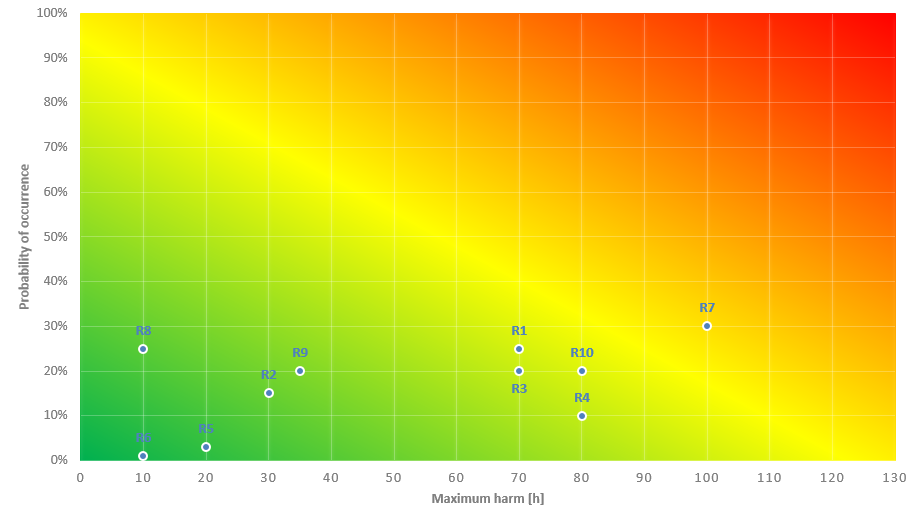
\includegraphics[width=1\textwidth]{img/riskmatrix}
	\caption{Risk Matrix}
	\label{fig:Risk Maxtrix}
\end{figure}
\section{Systemsetup}
This chapter details the infrastructure that was used in this project. It includes the local setup on the developer machines as well as all remote infrastructure such as continuous integration and project management tools. 
\subsection{Local setup}
TexStudio 2.12\newline
Visual Studio Code 1.9\newline
Git 


\subsection{Server setup}
Jira \newline
Bamboo\newline
NodeJS\newline
SonarQube\newline
Postgres

\subsubsection{Project homepage}
In order to alway be fully aware about all aspects of the project, it was decided to setup a small project homepage that gathers all relevant information and displays it at a single point. This was done to support the authors with their work, but also to provide a real-time insight to the advisors of this project. \newline
The first abstract of the page collects all links that are relevant to the project. This includes all code repositories, but also links to all project management tools used as well as to the documentation of this project.  \newline
\begin{figure}[H]
	\centering
	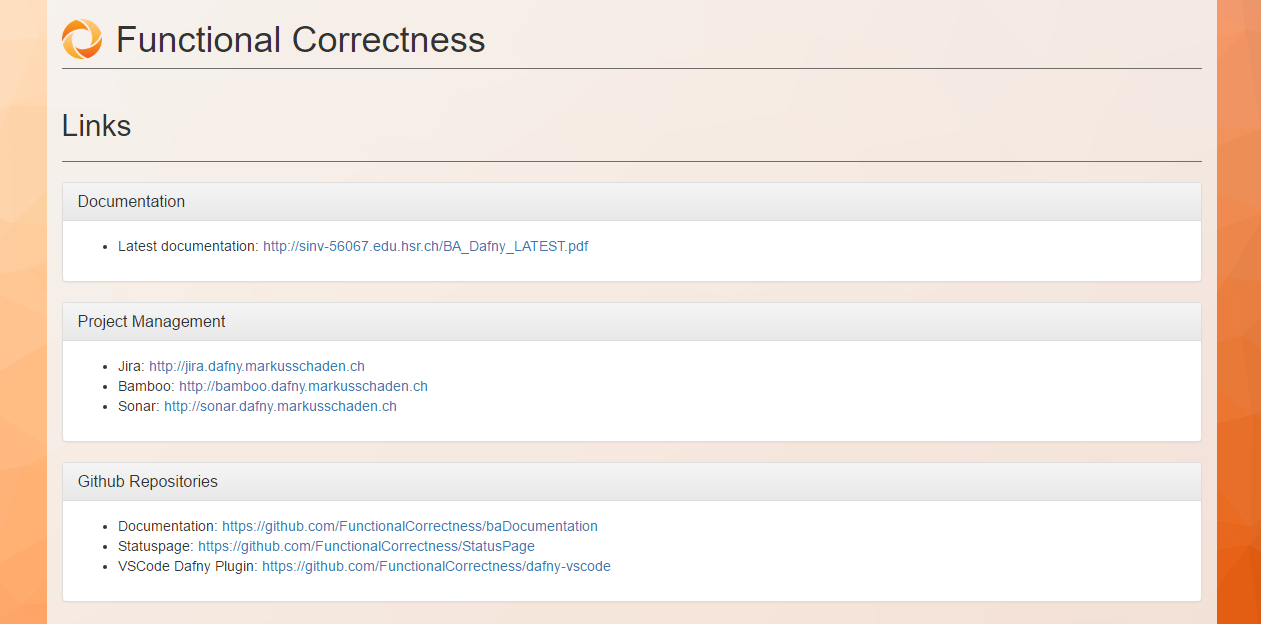
\includegraphics[width=1\textwidth]{img/homeLinks}
	\caption{All links relevant to the project}
	\label{fig:Project Links}
\end{figure}

Since continuous integration was ingrained to this project from the start, the last stable version of the plugin was continuously available in the marketplace of Visual Studio Code. To keep track of how many people are already using the plugin, a counter displaying the downloads was added to the home page. \newline
\begin{figure}[H]
	\centering
	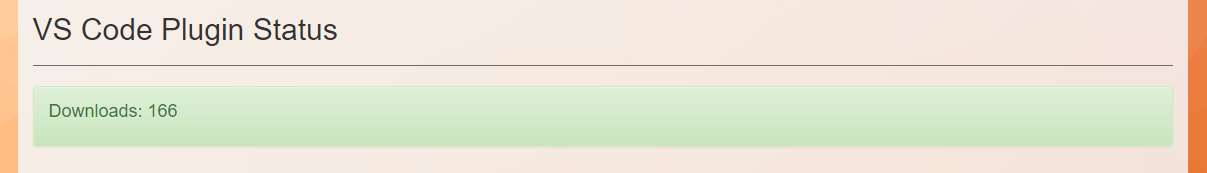
\includegraphics[width=1\textwidth]{img/homeCounter}
	\caption{Downloads of the plugin}
	\label{fig:Plugin Downloads}
\end{figure}

As already mentioned, it was paramount to this project to implement continuous integration, not only with the plugin, but for all other artifacts as well (the home page itself, or the documentation). In order to achieve this, various test- and build jobs were defined with Bamboo. To quickly see if anything is amiss, the home page also displays the status of these tasks. \newline
\begin{figure}[H]
	\centering
	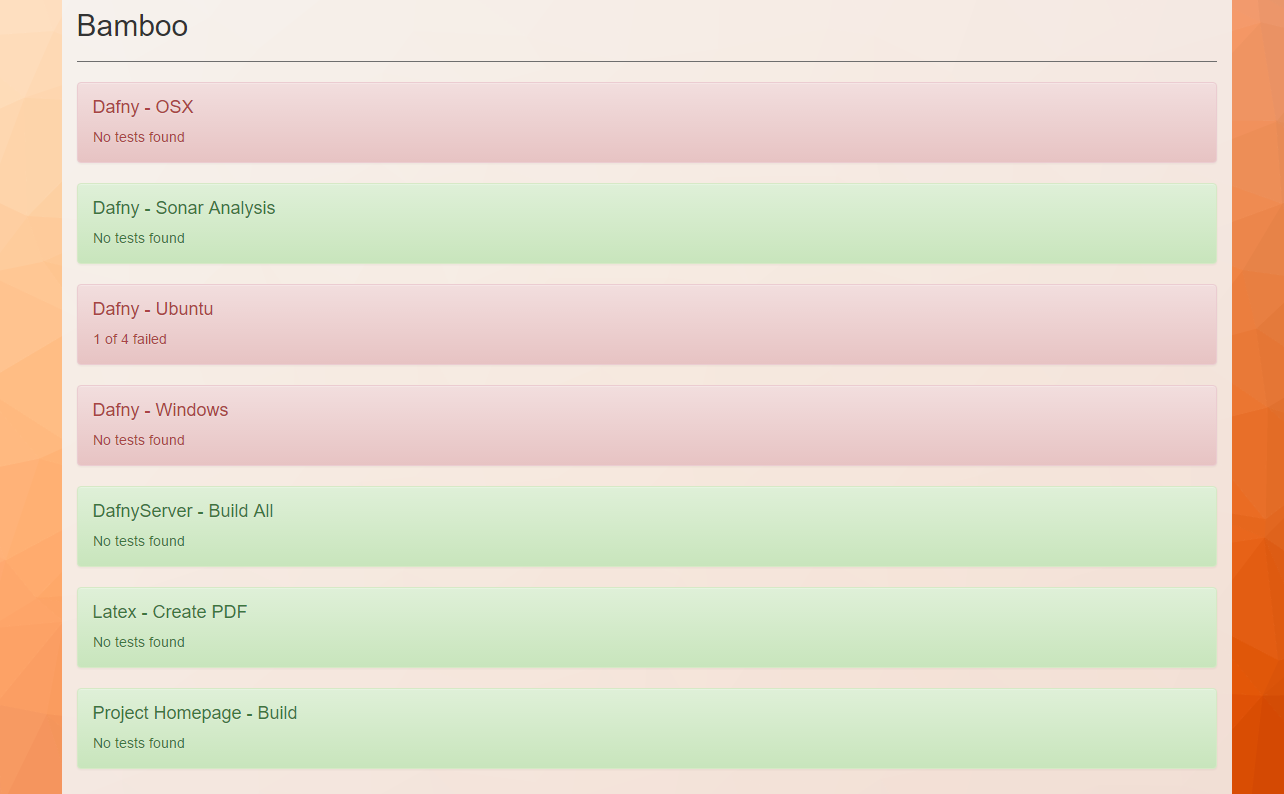
\includegraphics[width=1\textwidth]{img/homeBuilds}
	\caption{Status of all automated tasks}
	\label{fig:Bamboo Tasks}
\end{figure}

To keep code quality at a high level, SonarQube was used to analyze every commit to the code base of the plugin. The findings of SonarQube were also integrated into the home page. \newline
\begin{figure}[H]
	\centering
	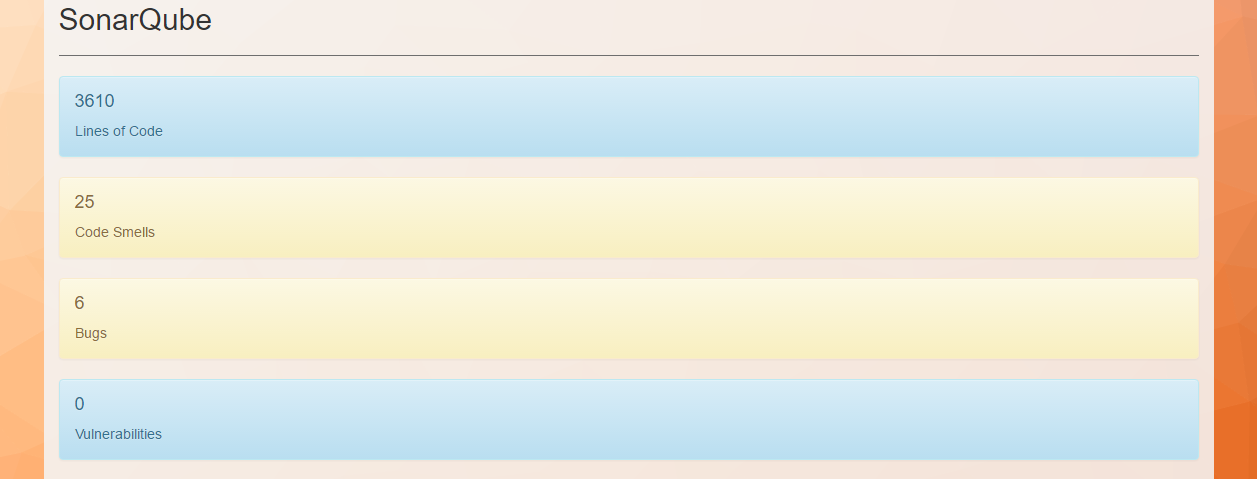
\includegraphics[width=1\textwidth]{img/homeSonar}
	\caption{Metrics analyzed by SonarQube}
	\label{fig:SonarQube}
\end{figure}

To support an iterative approach towards implementation, Scrum was chosen with weekly sprints. Tickets could either be new, worked upon or finished. To quickly grasp the work currently being done and how much time is planned for them, a dashboard displaying information from Jira, the project management tool used by this project, is also integrated into the home page.\newline
\begin{figure}[H]
	\centering
	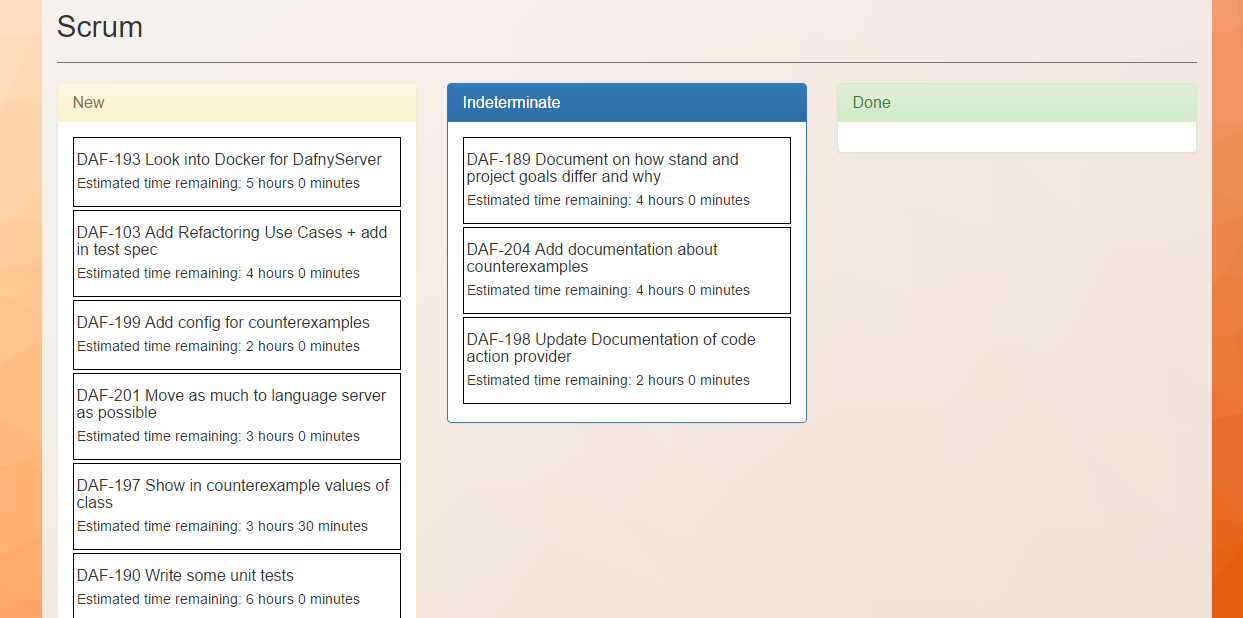
\includegraphics[width=1\textwidth]{img/homeScrum}
	\caption{Project Dashboard from Jira}
	\label{fig:Jira}
\end{figure}

Lastly, it was important to stay on track during the project regarding time management. To have a simple overview on the time invested, an additional import from Jira was done, which is implemented as graph detailing the cumulative amount of hours worked on the project. \newline
\begin{figure}[H]
	\centering
	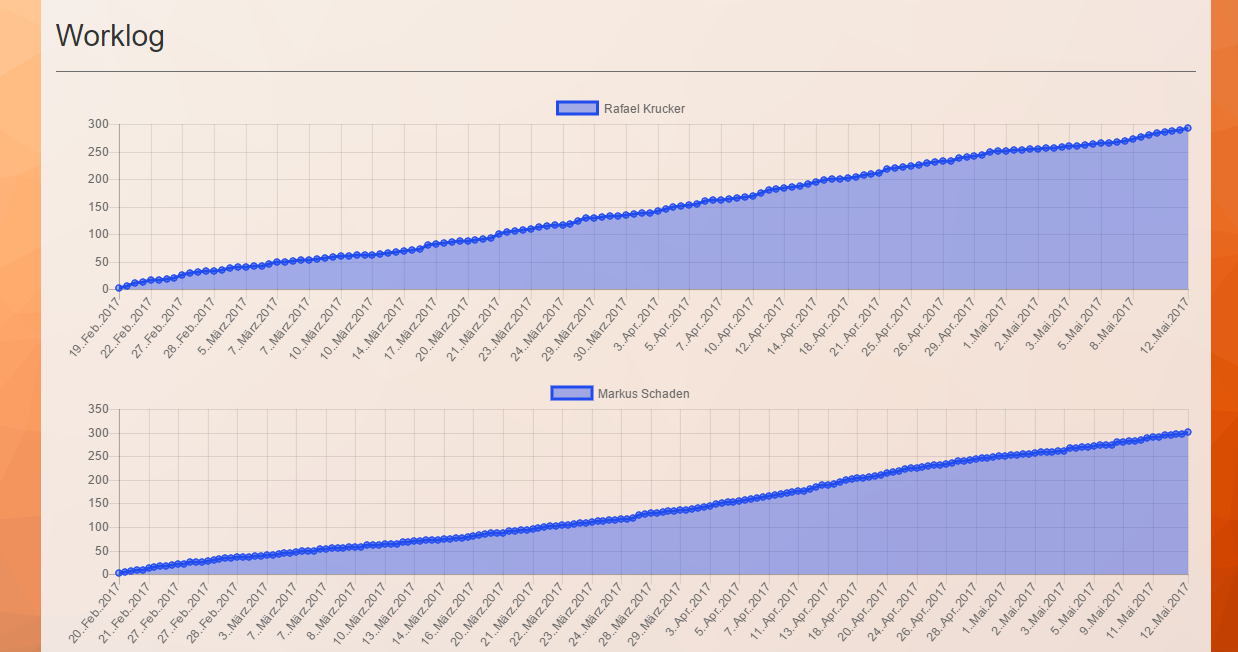
\includegraphics[width=1\textwidth]{img/homeTime}
	\caption{Hours worked on the project}
	\label{fig:Jira Hours}
\end{figure}

Together, all these abstracts give a detailed overview of the project, allowing for a quick grasp of the work being done, its quality and how the project is coming along over time. It was often the first point of action to open the page when working on the project. 


\subsection{Continuous Integration}

To ensure that the code quality is high and the code is working as expected, all commits trigger automated builds of the respective project. A commit to the documentation repository executes a job which creates a file out of the \LaTeX sources. This document is then copied to the \emph{wwwroot} directory, which then can be downloaded from the project homepage. Commits to the vscode-dafny repository will result in a build and a complete run of all tests on the three environments afterwards. Therefore remote agents are installed on Ubuntu and OSX , which test the plugin on these operation system.  Additionally SonarQube is used to find bugs and bad practices as early as possible. The last repository which triggers a bamboo job is the project homepage. The latest version is built and deployed when a commit is performed. 


\begin{figure}[H]
	\centering
	\includegraphics[width=1\textwidth]{img/ci}
	\caption{Server Setup}
	\label{fig:Server setup}
\end{figure}
\section{Conception and Design}
This chapter documents the most important design decisions and the rationale behind them.


\subsection{Contract generation examples} \label{examples}
Since Dafny offers built-in specification constructs, a programmer would greatly benefit from generation of contracts for common situations. This chapter first introduces three examples in programming, that could be made safer through the use of contracts. The solution is then generalized in order to be more widely applicable.
\subsubsection{Example 1: Array access} \label{Example 1}

\paragraph{Problem:}

A method accesses an array with an index, which is given as a parameter. The array may be a field or also be a parameter. The array may be null or the index may be out of bound.
\paragraph{Solution:}
Generate a precondition which checks if the array is not null and the index is in bound of the array.

\paragraph{Code:}
\begin{lstlisting}[language=dafny]
method FindUsafe(a: array<int>, key: int) return (element: int)
{
	return a[key];
}

method FindSafe(a: array<int>, key: int) return (element: int)
	requires a != null && 0 <= key < a.Length
{
	return a[key];
}
\end{lstlisting}



\subsubsection{Example 2: Simple domain specific constraints} \label{Example 2}
\paragraph{Problem:}
A method that processes withdraws form a bank account may not make a bank balance negative.
\paragraph{Solution:}
Generate a pre- and postconditions on methods which modify relevant fields, according to domain specific constraints.

\paragraph{Code:}
\begin{lstlisting}[language=dafny]
class BankAccountUnsafe {
	var balance: int;
	
	method withdraw(amount: int) modifies this {
		balance := balance - amount;
	}
}

class BankAccountSafe {
	var balance: int;
	
	method withdraw(amount: int) 
		requires balance >= amount  
		ensures balance >= 0  
	modifies this {
		balance := balance - amount;
	}
}
\end{lstlisting}


\subsubsection{Example 3: More complex Domain specific constraints} \label{Example 3}
\paragraph{Problem:}
A factory wants to model its processes. Their services consist of refining certain raw materials, which can interact aggressively with their machines. They have two types of machines, some which are subject to abreason over time, but also others which are very expensive and should not come into contact with aggressive materials. They want to make sure no aggressive materials come in contact with expensive machines under any circumstances.
\paragraph{Solution:}
Generate pre- and postconditions on methods which modify relevant fields, according to domain specific constraints.

\paragraph{Code:}
\begin{lstlisting}[language=dafny]

class RawMaterial {
	var abreasesMachines: bool;
}

class NormalMachine {
	var prestine: bool;
	constructor() modifies this {
		this.prestine := true;
	}
	method refineMatieral(material: RawMaterial) {
		...
	}
	method processMaterial(material: RawMaterial) 
		requires material != null
	modifies this {
		this.refineMatieral(material);
		this.prestine := !material.abreasesMachines;
	}
}

class ExpensiveMachine {
	var prestine: bool;
	constructor() modifies this {
		this.prestine := true;
	}
	
	method refineMatieral(material: RawMaterial) {
	
	}
	
	method processMaterial(material: RawMaterial) 
		requires material != null
		requires !material.abreasesMachines
		ensures prestine
	modifies this {
		this.refineMatieral(material);
		this.prestine := !material.abreasesMachines;
	}
}
\end{lstlisting}

\subsubsection{Underlying problems}
All three examples have in common, that without the correct preconditions, they should result in proof obligations which cannot be proven.
This subsection first details three common concepts that occur when reasoning about proof obligations. The next subsection sets them into connections with the problems mentioned in \ref{examples}.

\paragraph{Application of partial functions} \label{partial function}
One of the three problems can be expressed as the application of partial functions, which are defined by the following three objects:
\begin{itemize}
	\item A set A called the input set of the function
	\item A set B called the output set of the function.
	\item A rule f that transforms some elements of A to some elements of B such that no element a from A is transformed to more than one element of B.\cite[197]{khoussainov}
\end{itemize}
The definition states that not all input values may be mapped by the function. The problem here therefore is to ensure that the function is applied on only a valid subset of A.


\paragraph{Invariants} \label{invariants}
An Invariant can be defined as follows: A quantity which remains unchanged under certain classes of transformations. Invariants are extremely useful for classifying mathematical objects because they usually reflect intrinsic properties of the object of study.\cite[282ff]{hunt}
\newline An Invariant is therefore extremely useful when one wants to ensure certain conditions of an object, which must hold at all times. If an invariant is to be applied to an object with multiple attributes, it is usually defined as a postconditions on all attributes. 

\paragraph{Non provable Goals} \label{non provable goal}
These are situations that are impossible to prove, because some preconditions do not hold or not sufficient information is available. They are very hard to detect and isolate from provable goals, although some work has found solutions under certain restrictions, for instance \cite{goals}. When an unprovable goal is encountered in a context, it is much easier to simply state it as a precondition for the context to be valid, thus burdening the calling context with ensuring that the goal holds. 

\subsubsection{Solving the problems in an abstract way}
This subsection finally shows how the patterns detailed above can be used to solve the programming examples, thus allowing generic solutions for many similar problems.

\paragraph{Problem 1}
The situation shown in \ref{Example 1} is a very common situation while programming, basically one wants to prove that the index is always in the bounds of the array. Accessing an element in an array is an example of the \nameref{partial function}, where the set A only goes from zero to the length of the array minus one. Therefore one would have to prove that the application of the partial function does not result in an invalid element being given as an argument. The expression, which is used to get access, can be arbitrarily complex. The computation to ensure the in-boundness can be very expensive.  \newline
Also the second pattern discussed in \nameref{invariants} could be applied, always ensuring that a given parameter is in bound of an array of an object, although this would not work with how invariants are normally applied, namely as postconditions. Since the expression that generates the index has nothing to do with the object itself, it is questionable if this is the right pattern to apply to this situation. \newline
The third pattern, discussed in \nameref{non provable goal}, works very well if one assumes that it can't be proven that the expression will always lead to a successful application of the partial function (although it could be proven in many cases). This allows to define this property as a precondition of the method, thus shifting the burden to the caller to always check his arguments. This is an easy and feasible solution to the first problem. 

\paragraph{Problem 2} \label{Problem 2}
The example in \ref{Example 2} is an example of a domain specific limitation where a bank account's balance should never fall below zero. In this specific implementation the usage of \nameref{partial function} could be discussed, since it is implemented as a binary minus function which only allows subtrahends from a certain range, although this approach could not be used for all possible implementations and is therefore not a feasible solution. \newline
The second pattern discussed in \nameref{invariants} best describes the semantics of the situation in a very general way, it could simply be stated as an invariant, that the balance has always to be positive. This does not suffice though, as it does not isolate the parts yet which could break the invariant. \newline
The third pattern, discussed in \nameref{non provable goal}, works very well in conjunction with the second one. All sub goals that should hold so that the invariant holds, in this case that the amount should be smaller than the balance, can be viewed as unprovable goals in this context. They can be therefore be formulated as preconditions such that the caller has the burden of applying correct arguments to the function. This practice isolates the parts which could break the invariant, allowing to write the function as safe as possible.

\paragraph{Problem 3}
The example in \ref{Example 3} is also an example of a domain specific limitation, although more complex. It combines several classes together, which could also potentially be subtyped The goal is to never let an expensive machine be subjected to abreason, therefore only allowing non-aggressive raw materials as input. In this specific implementation the usage of \nameref{partial function} could work very well, since the input set of the partial function is very small, namely only the value true on the abreasesMachines property of a raw material However, if we extend the hierarchy of materials and implement the calculation of abreasesMachines differently, it is unclear if all cases could be computed efficiently. \newline
The second pattern discussed in \nameref{invariants} best describes the semantics of the situation in a very general way, it could simply be stated as an Invariant, that the pristine property on the expensive machine is always true. This does not suffice though, as it does not isolate the parts yet which could break the invariant. This is the same situation as in \nameref{Problem 2} \newline
The third pattern could be used much the same way as in \nameref{Problem 2}. The condition, that the raw material may never abrease machines, can be written as a precondition and together with the usage of invariants holds the greatest amount of security regarding the domain constraints.

\subsubsection{Conclusion}
As the discussion above shows, all of the three problems can be solved through the application of \nameref{invariants} and \nameref{non provable goal}. They make it unnecessary to solve the problems of \nameref{partial function}, which is often harder to do. All occurrences, where such a computation would be needed, can be seen as non provable goals and stated as preconditions for a method. The usage of invariants offers a syntactical transparent way of describing domain specific rules, and the implementation is a relative simple one, as it just is translated into postconditions for all methods of an object. Together these two techniques offer solutions to many different problems in computer science, since they operate on a high abstraction, while still being syntactical transparent.\newline 
In the first example, the language itself has enough domain knowledge in order to generate the unprovable proof obligations, since it knows about the array type and its restrictions. In the two other cases the language  needs more domain knowledge in order to generate the unprovable proof obligations. As was shown above, invariants are a good way of providing this domain knowledge.
Once the unprovable proof obligations can be found, they can be used as hints for preconditions that can be suggested to the programmer.\newline
The hardest part of the implementation is the identification of non provable subgoals that are in relation to an invariant. To do this, detailed knowledge has to be available of the control flow of a program and all possible outcomes of a computation have to be considered, although the problem can be relaxed if one allows for false positives in the identification of non provable subgoals. Since the plugin only offers refactorings and does not apply them automatically, the programmer still can decide if the setting of the non provable goal as precondition is necessary.  


\subsection{Test specification}

\subsubsection{Unit Tests}
Visual Studio Code plugins can be tested with standard javascript testing frameworks like Mocha or Jasmine, if they don't use any features of Visual Studio Code itself. This allows to test core logic without the need to run tests inside VS Code.

\subsubsection{Integration Tests}
Visual Studio Code extensions which require VS Code API can be tested with help of a special instance of Visual Studio Code. Inside this instance, the extension can use the full API and tests can execute commands like creating a new file, entering a character, using autocompletion and verifying if the extension works as expected.   

\subsubsection{Test overview}
To verify that the Dafny Visual Studio Code Plugin is working as expected, it has to be properly tested. Two possibilities exist. Either automatic unit / integration tests or manual testing. The best would be to test everything automatically. Unfortunately this is not possible, since although the Visual Studio Code Test API provides a rich set of methods, there is no direct access to the file system or a possibility to wait for certain tasks to finish. For this reason some tests have to be performed manually, especially use cases which install Dafny and rely heavily on scripts. On the other side, if all automatic tests fail, it's mostly a clear signal that something with the server is not okay. So the automatic tests also verify if the DafnyServer is working correctly. During development it is also quite easy to verify certain features on the fly. 
Below one first finds what is tested and how, followed by a table which explains how the individual use cases are tested and guides for manual testing. 

\subsubsection{System Tests}
As discussed in the last chapter, not everything can be easily tested, so the test scope has to be restricted. The following table shows which system component are tested and how.
\begin{longtable}{ p{0.3\textwidth} | p{0.2\textwidth} | p{0.4\textwidth} }
\textbf{Topic} & \textbf{Tested} & \textbf{Description}\\
	Installation of Dafny plugin & Manual & Manual installation of Dafny and setting of base path   \\
	Automatic installation of Dafny & Manual & Easier to validate that base path is set correctly and all files exists \\
	Uninstallation of Dafny & Manual & Verify on file system level\\
	Communication DafnyServer and Dafny plugin & Manual + Automatic & Test if output from DafnyServer is correctly parsed and displayed\\
	Restart DafnyServer task & Manual & Check if a new PID is used and the other is stopped\\
	Local queue & Manual & DafnyServer can be paused in Visual Studio Code and queuing can be checked \\
	Syntax highlighting & Manual & Look on our examples \\
	Verification on typing & Manual & Easy to test manually\\
	Snippets & Manual & Check if snippets are working\\
	Document symbol provider & Automatic & Can easily be tested with the Visual Studio Code API \\
	Hover Provider & Automatic & Can easily be tested with the Visual Studio Code API\\
	Definition Provider & Automatic & Can easily be tested with the Visual Studio Code API  \\
	Code Lens & Automatic & Can easily be tested with the Visual Studio Code API\\
	Automatic generation of contracts & Manual & \todo{add desc} \\
	Autocompletion for identifiers & Automatic & \todo{add desc} \\
	Reporting of Dafny best practices violations & Manual & \todo{add desc} \\
\end{longtable}


\subsubsection{Basic tests}
If the Dafny plugin is installed, the following procedure is expected inside Visual Studio Code. 
\begin{itemize}
\item The Dafny language is available
\item .dfy is associated with the Dafny plugin
\item Asks to install Dafny, if no DafnyServer is found 
\item Starts the DafnyServer if a .dfy is opened
\item Verification status of a .dfy file is shown
\item Assertion errors are reported
\end{itemize}

\subsubsection{Detailed manual tests}
The following paragraphs explain how a certain feature can be tested manually, which steps have to be performed and what the expected result should be.

\paragraph{Manual installation}
\textbf{\newline Steps:}
\begin{enumerate}
\item Uninstall the plugin and remove Dafny (/home/.Dafny or \%AppData\%/Roaming/Dafny)
\item Remove the entry "dafny.basePath" from the user configuration file 
\item Restart Visual Studio Code - There should be an error that Dafny is not installed
\item Install Dafny from \href{https://github.com/FunctionalCorrectness/dafny-microsoft/releases}{https://github.com/FunctionalCorrectness/dafny-microsoft/releases}
\item Set "dafny.basePath" to the extracted archive location
\item Open the file simpleTest.dfy
\item Execute "Dafny: RestartServer" task
\end{enumerate}
\textbf{\newline Expected:}
The DafnyServer should be started and the file verified. This can be seen in the status bar. On the right side, there should be the PID of the DafnyServer and on the left side the status "Verified"

\paragraph{Status change}
\textbf{\newline Steps:}
\begin{enumerate}
	\item Open the file invalidAsserts.dfy

\end{enumerate}
\textbf{\newline Expected:}
The server should first start and afterwards the status should display "Verifiying". After the DafnyServer verified the program, the status should have been changed to "Not Verified" and multiple asserts are marked red. 

\paragraph{Server crash}
\textbf{\newline Steps:}
\begin{enumerate}
	\item Open the file simpleTest.dfy
	\item The server should be started and the file verified
	\item Kill the DafnyServer process
\end{enumerate}
\textbf{\newline Expected:}
The server should restart automatically, with a corresponding message shown inside Visual Studio Code. 


\paragraph{Local queue}
\textbf{\newline Steps:}
\begin{enumerate}
	\item Open the file simpleTest.dfy
	\item The server should be started and the file verified
	\item Open Visual Studio Code and attach the debugger to the DafnyServer process
	\item Set a breakpoint in the verify method
	\item Change a assert in the simpleTest.dfy 
	\item Visual Studio Code should break at the breakpoint
	\item Open more files
\end{enumerate}
\textbf{\newline Expected:}
The queue size should be getting bigger and bigger as new files are opened. After the breakpoint is removed and the debugger detached, the queue size should decreasing. 

\paragraph{Verification on typing}
\textbf{\newline Steps:}
\begin{enumerate}
	\item Open the file simpleTest.dfy
	\item Change a assert that it does not hold (in under 0.7 seconds)
\end{enumerate}
\textbf{\newline Expected:}
After 0.7 seconds (default value) the file should be verified and the error should be displayed 

\paragraph{Automatic installation}
\textbf{\newline Steps:}
\begin{enumerate}
\item Uninstall the Server with "Dafny: Uninstall DafnyServer" task
\item Restart Visual Studio Code - There should be an error that Dafny is not installed
\item Open the file simpleTest.dfy
\item Install Dafny with the task "Dafny: Install DafnyServer" 
\end{enumerate}
\textbf{\newline Expected:}
Dafny should be downloaded, extracted, started and the file verified. See UC1, UC2, UC3 Expected


\paragraph{Uninstallation}
\textbf{\newline Steps:}
\begin{enumerate}
	\item Uninstall the Server with "Dafny: Uninstall DafnyServer" task
\end{enumerate}
\textbf{\newline Expected:}
Dafny should be uninstalled from the system. /home/.Dafny or \%AppData\%/Roaming/Dafny should be empty.


\paragraph{Snippets}
\textbf{\newline Steps:}
\begin{enumerate}
	\item Open the source code file snippets/dafny.json and remember a prefix from the list
	\item Enter the prefix 
	\item Press Enter
\end{enumerate}
\textbf{\newline Expected:}
The snippet should be inserted and can be edited


\paragraph{Autocompletion for identifiers}
Autocompletion can be tested with the Visual Studio Code Test API. For this, a file is loaded with a set of methods. Afterwards, some test check if the existing methods are considered for autocompletion. Additionally, more refactoring tests will be performed under this use case. 


\section{Dafny VSCode}
Github Repository: \href{https://github.com/FunctionalCorrectness/dafny-vscode}{https://github.com/FunctionalCorrectness/dafny-vscode}

\subsection{Overview}
\todo{Maybe add a class diagram}

\subsection{Visual Studio Code Plugin}
\subsubsection{Structure}
When a Visual Studio Code plugin is implemented as a language server, the plugin consists of two parts. The first one is an IDE-agnostic language server, which is further explained in \ref{langServer}. The second part is the actual plugin which interacts with Visual Studio Code and relies on the language server to provide functionality. \newline
The actual plugin will further on be referenced as the client part of the plugin. The most important part of the client part is a file called package.json. It informs the IDE about the following points:
\paragraph{Activation}
Details for what the plugin is designed and when it is activated. Normally, plugins stay dormant until a use case is triggered for which they are needed. For this project, this is the case whenever a Dafny file is opened in Visual Studio Code.

\paragraph{Commands}
Details which commands this plugin exposes. Next to standard callbacks such as when a file is first opened or saved, additional custom commands can be registered here. This projects exposes some custom commands such as to install the Dafny server or check the version of the server currently installed. This also includes key bindings for the registered commands.

\paragraph{Configuration}
Is used to configure a plugin. For this project this for instance entails the path to the Dafny executable or if it is running on a .NET or mono environment. It also sets Visual Studio Code specific configuration, such as how long of a delay should follow typing before the file is reevaluated.

\paragraph{Dependencies}
Details all the dependencies in the form of node modules that the plugin has.

\paragraph{Meta information}
Additionally, this section details meta information about the plugin such as who developed it, which version it has and so on.


\todo{Further explanation about the client side of the plugin}


\section{Language Server Protocol}\label{langserver}
Visual Studio Code plugins can be implemented in two ways: the first one is via the standard Visual Studio Code API and the second one is in form of a language server. Language servers follow a standard protocol to provide services for working with different programming languages and offer often used features such as go to definition. While this offers great portability and easy integration with other IDEs or tools that work with language servers, the implementation as a language server was at first rejected in this project. \newline
The main reason was that the project extends an existing plugin, which was already built around the standard Visual Studio Code API. A second consideration was that the usage of language servers in Visual Studio Code plugins is very sparse at the moment. The big language integrations like typescript or javascript do not implement their plugins as language servers, while the GoLang plugin offers experimental support at this time. The not wide spread usage in this environment was therefore another reason to not implement a language server initially. \newline
However, during the process of implementing the project, many features were faster done than initially estimated, and other planned features were proven to not be feasible for the scope of this work. This meant that more time could be spend on features or ideas that were labeled as optional in the beginning. Since the concept of a language server itself is intriguing due to the potential to widen the user base considerably, it was decided to try to restructure the plugin as a language server. \newline
The restructuring only took about 30 hours since the plugin was already nicely programmed in regard to separation of concerns, such that only a wrapper had to be written that implements the language server protocol and redirects the requests to the components that implement the core functionality. 
Since the plugin now is programmed in form of a language server, it can potentially easily be used in other IDEs such as Eclipse or Emacs once they fully implement the language server protocol on their side. In hindsight it is thought that the change of the original decision and the additional work that had to be done was well worth regarding the resulting outcome. \newline
Below a short overview of the protocol and how it was implemented is given. Server here refers to the language server and not the DafnyServer. The later one is explicitly written as DafnyServer.

\subsection{The protocol}
The Language Server protocol is used between a tool (the client) and a language smartness provider (the server) to integrate features like auto complete, goto definition, find all references and alike into the tool. \cite{langserver} \newline
The language server maintains semantic information about a program implemented in a particular language. The language server is notified whenever the user opens a document in the tool. Also edits by the user are reported, so the language server is notified of the changes and can update the program's semantic information. Currently, only point to point communication is supported by the protocol. Sharing one language server between multiple tools would require further protocol mechanisms like locking a file.\newline
One of the most basic features is the analysis of the document and generation of errors and warnings (called diagnostics by Microsoft), which the tool then can display. Furthermore, more sophisticated features are also provided. For instance, the client can send a definition request for a symbol to the server. The server is then tasked to answer with the URI of the file and the range in that file where the definition can be found. The tool is then free to open said file or simply provide a peek at it through an overlay. \newline
\begin{figure}[H]
	\centering
	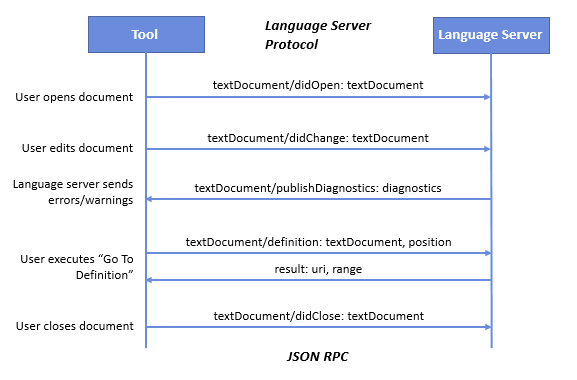
\includegraphics[width=1\textwidth]{img/langServerOverview}
	\caption{Example of the communication between the client and the server}
	\label{fig:langserveroverview}
\end{figure}
The server also gets notified when the user closes a file. An important distinction to make is that whenever the client has opened a file, it resides in memory and the tool maintains it. When it is closed, it simply lies in the file system like any other file. \newline
The communication between the tool and the language server uses JSON RPC v2.0. Language servers can implement an arbitrary subset of features defined in the protocol, so in the first response by the server it details what capabilities it has. \newline
\subsection{Communication Types}
There are two different types to communicate between the client and the server. It's either a notification or a request. 
\paragraph{Notification}
A notification is just a message which can be sent in both directions. But one can't wait for an answer. These types of messages are mostly used to inform the partner that something happened. 
\paragraph{Request}
A request on the other side is a message which will be answered.  
\subsection{Standard Implementation}
Next to custom commands, which are explained in chapter \ref{custom commands} and following, the language server describes a standardized API \cite{protMaster} for features that are useful when working with a language server. The API is designed as a Request / Reply Protocol. Below a list of the implemented Requests is listed, while a detailed description on how the implementation was done can be found in \ref{architecture}. All the structures detailed in this chapter are defined by the protocol. \newline
\paragraph{Message Structure}
The protocol describes how the messages exchanged between the client and the server must be structured. A generic example of a request and a response are as follows:
\textbf{Request}
\begin{lstlisting}[language=json,firstnumber=1]
interface RequestMessage extends Message {

  /**
  * The request id.
  */
  id: number | string;

  /**
  * The method to be invoked.
  */
  method: string;

  /**
  * The method's params.
  */
  params?: any
}
\end{lstlisting}
\textbf{Response}
\begin{lstlisting}[language=json,firstnumber=1]
interface ResponseMessage extends Message {
  /**
  * The request id.
  */
  id: number | string | null;

  /**
  * The result of a request. This can be omitted in
  * the case of an error.
  */
  result?: any;

  /**
  * The error object in case a request fails.
  */
  error?: ResponseError<any>;
}

interface ResponseError<D> {
  /**
  * A number indicating the error type that occurred.
  */
  code: number;

  /**
  * A string providing a short description of the error.
  */
  message: string;

  /**
  * A Primitive or Structured value that contains additional
  * information about the error. Can be omitted.
  */
  data?: D;
}

export namespace ErrorCodes {
  // Defined by JSON RPC
  export const ParseError: number = -32700;
  export const InvalidRequest: number = -32600;
  export const MethodNotFound: number = -32601;
  export const InvalidParams: number = -32602;
  export const InternalError: number = -32603;
  export const serverErrorStart: number = -32099;
  export const serverErrorEnd: number = -32000;
  export const ServerNotInitialized: number = -32002;
  export const UnknownErrorCode: number = -32001;

  // Defined by the protocol.
  export const RequestCancelled: number = -32800;
}
\end{lstlisting}
\paragraph{Data structures}
Next, an overview over the most commonly used data structures used in the protocol is given: \newline
\textbf{Position}
Describes a position, e.g. of a cursor, in a document.
\begin{lstlisting}[language=json,firstnumber=1]
interface Position {
  /**
  * Line position in a document (zero-based).
  */
  line: number;

  /**
  * Character offset on a line in a document (zero-based).
  */
  character: number;
}
\end{lstlisting}
\textbf{Range}
Describes an area in a document which can span multiple lines of text.
\begin{lstlisting}[language=json,firstnumber=1]
interface Range {
  /**
  * The range's start position.
  */
  start: Position;

  /**
  * The range's end position.
  */
  end: Position;
}
\end{lstlisting}
\textbf{Location}
Describes a location inside a resource, such as a line inside a text file.
\begin{lstlisting}[language=json,firstnumber=1]
interface Location {
  uri: DocumentUri;
  range: Range;
}
\end{lstlisting}
\textbf{Diagnostic}
Describes a diagnostic such as an error or a compiler warning.
\begin{lstlisting}[language=json,firstnumber=1]
interface Diagnostic {
  /**
  * The range at which the message applies.
  */
  range: Range;

  /**
  * The diagnostic's severity. Can be omitted. If omitted it is up to the
  * client to interpret diagnostics as error, warning, info or hint.
  */
  severity?: number;

  /**
  * The diagnostic's code. Can be omitted.
  */
  code?: number | string;

  /**
  * A human-readable string describing the source of this
  * diagnostic, e.g. 'typescript' or 'super lint'.
  */
  source?: string;

  /**
  * The diagnostic's message.
  */
  message: string;
}
\end{lstlisting}
\textbf{Server capabilities}
With this data structure, the server can tell the client which features it implements. 
\begin{lstlisting}[language=json,firstnumber=1]
interface ServerCapabilities {
  /**
  * Defines how text documents are synced. Is either a detailed structure defining each notification or
  * for backwards compatibility the TextDocumentSyncKind number.
  */
  textDocumentSync?: TextDocumentSyncOptions | number;
  /**
  * The server provides hover support.
  */
  hoverProvider?: boolean;
  /**
  * The server provides completion support.
  */
  completionProvider?: CompletionOptions;
  /**
  * The server provides signature help support.
  */
  signatureHelpProvider?: SignatureHelpOptions;
  /**
  * The server provides goto definition support.
  */
  definitionProvider?: boolean;
  /**
  * The server provides find references support.
  */
  referencesProvider?: boolean;
  /**
  * The server provides document highlight support.
  */
  documentHighlightProvider?: boolean;
  /**
  * The server provides document symbol support.
  */
  documentSymbolProvider?: boolean;
  /**
  * The server provides workspace symbol support.
  */
  workspaceSymbolProvider?: boolean;
  /**
  * The server provides code actions.
  */
  codeActionProvider?: boolean;
  /**
  * The server provides code lens.
  */
  codeLensProvider?: CodeLensOptions;
  /**
  * The server provides document formatting.
  */
  documentFormattingProvider?: boolean;
  /**
  * The server provides document range formatting.
  */
  documentRangeFormattingProvider?: boolean;
  /**
  * The server provides document formatting on typing.
  */
  documentOnTypeFormattingProvider?: DocumentOnTypeFormattingOptions;
  /**
  * The server provides rename support.
  */
  renameProvider?: boolean;
  /**
  * The server provides document link support.
  */
  documentLinkProvider?: DocumentLinkOptions;
  /**
  * The server provides execute command support.
  */
  executeCommandProvider?: ExecuteCommandOptions;
  /**
  * Experimental server capabilities.
  */
  experimental?: any;
}
\end{lstlisting}

\paragraph{Implemented Requests}
Next, pairs of Request / Responses implemented by this project are listed:
\textbf{Shutdown Request}
The shutdown request is sent from the client to the server. It asks the server to shut down, but to not exit (otherwise the response might not be delivered correctly to the client). There is a separate exit notification that asks the server to exit.

\textbf{Request}
\begin{lstlisting}[language=json,firstnumber=1]
  method: 'shutdown'
  params: void
\end{lstlisting}
\textbf{Response}
\begin{lstlisting}[language=json,firstnumber=1]
result: null
error: code and message set in case an exception happens during shutdown request.
\end{lstlisting}

\textbf{Exit Notification}
A notification to ask the server to exit its process. The server should exit with success code 0 if the shutdown request has been received before; otherwise with error code 1.

\textbf{Notification}
\begin{lstlisting}[language=json,firstnumber=1]
method: 'exit'
params: void
\end{lstlisting}

\textbf{ShowMessage Notification}
The show message notification is sent from a server to a client to ask the client to display a particular message in the user interface.

Notification:
\begin{lstlisting}[language=json,firstnumber=1]
method: 'window/showMessage'
params: ShowMessageParams defined as follows:
interface ShowMessageParams {
  /**
  * The message type. See {@link MessageType}.
  */
  type: number;
	
  /**
  * The actual message.
  */
  message: string;
}
\end{lstlisting}
\textbf{ShowMessage Request}
The show message request is sent from a server to a client to ask the client to display a particular message in the user interface. In addition to the show message notification the request allows to pass actions and to wait for an answer from the client.

Request:
\begin{lstlisting}[language=json,firstnumber=1]
method: 'window/showMessageRequest'
params: ShowMessageRequestParams
\end{lstlisting}
Response:
\begin{lstlisting}[language=json,firstnumber=1]
result: the selected MessageActionItem
error: code and message set in case an exception happens during showing a message.
interface ShowMessageRequestParams {
  /**
  * The message type. See {@link MessageType}
  */
  type: number;
	
  /**
  * The actual message
  */
  message: string;
	
  /**
  * The message action items to present.
  */
  actions?: MessageActionItem[];
}
\end{lstlisting}

\textbf{DidChangeConfiguration Notification}

A notification sent from the client to the server to signal the change of configuration settings.

Notification:
\begin{lstlisting}[language=json,firstnumber=1]
method: 'workspace/didChangeConfiguration',
params: DidChangeConfigurationParams defined as follows:
interface DidChangeConfigurationParams {
  /**
  * The actual changed settings
  */
  settings: any;
}
\end{lstlisting}

\textbf{DidOpenTextDocument Notification}

The document open notification is sent from the client to the server to signal newly opened text documents. The document's truth is now managed by the client and the server must not try to read the document's truth using the document's Uri.

Notification:
\begin{lstlisting}[language=json,firstnumber=1]
method: 'textDocument/didOpen'
params: DidOpenTextDocumentParams defined as follows:
interface DidOpenTextDocumentParams {
  /**
  * The document that was opened.
  */
  textDocument: TextDocumentItem;
}
\end{lstlisting}

\textbf{DidChangeTextDocument Notification}

The document change notification is sent from the client to the server to signal changes to a text document. In 2.0 the shape of the params has changed to include proper version numbers and language ids.

Notification:
\begin{lstlisting}[language=json,firstnumber=1]
method: 'textDocument/didChange'
params: DidChangeTextDocumentParams defined as follows:
interface DidChangeTextDocumentParams {
  /**
  * The document that did change. The version number points
  * to the version after all provided content changes have
  * been applied.
  */
  textDocument: VersionedTextDocumentIdentifier;
	
  /**
  * The actual content changes.
  */
  contentChanges: TextDocumentContentChangeEvent[];
}
\end{lstlisting}

\textbf{DidCloseTextDocument Notification}

The document close notification is sent from the client to the server when the document got closed in the client. The document's truth now exists where the document's Uri points to (e.g. if the document's Uri is a file Uri the truth now exists on disk).

Notification:
\begin{lstlisting}[language=json,firstnumber=1]
method: 'textDocument/didClose'
params: DidCloseTextDocumentParams defined as follows:
interface DidCloseTextDocumentParams {
  /**
  * The document that was closed.
  */
  textDocument: TextDocumentIdentifier;
}
\end{lstlisting}

\textbf{PublishDiagnostics Notification}

Diagnostics notification are sent from the server to the client to signal results of validation runs.

Notification:
\begin{lstlisting}[language=json,firstnumber=1]
method: 'textDocument/publishDiagnostics'
params: PublishDiagnosticsParams defined as follows:
interface PublishDiagnosticsParams {
  /**
  * The URI for which diagnostic information is reported.
  */
  uri: DocumentUri;
	
  /**
  * An array of diagnostic information items.
  */
  diagnostics: Diagnostic[];
}
\end{lstlisting}
\textbf{Completion Request}

The Completion request is sent from the client to the server to compute completion items at a given cursor position. Completion items are presented in the IntelliSense user interface. If computing full completion items is expensive, servers can additionally provide a handler for the completion item resolve request ('completionItem/resolve'). This request is sent when a completion item is selected in the user interface. A typically use case is for example: the 'textDocument/completion' request doesn't fill in the documentation property for returned completion items since it is expensive to compute. When the item is selected in the user interface then a 'completionItem/resolve' request is sent with the selected completion item as a param. The returned completion item should have the documentation property filled in.

Request:
\begin{lstlisting}[language=json,firstnumber=1]
method: 'textDocument/completion'
params: TextDocumentPositionParams
\end{lstlisting}
Response:
\begin{lstlisting}[language=json,firstnumber=1]
result: CompletionItem[] | CompletionList
/**
* Represents a collection of [completion items](#CompletionItem) to be presented
* in the editor.
*/
interface CompletionList {
  /**
  * This list it not complete. Further typing should result in recomputing
  * this list.
  */
  isIncomplete: boolean;
  /**
  * The completion items.
  */
  items: CompletionItem[];
}
\end{lstlisting}

\textbf{Go to Definition Request}

The go to definition request is sent from the client to the server to resolve the definition location of a symbol at a given text document position.

Request:
\begin{lstlisting}[language=json,firstnumber=1]
method: 'textDocument/definition'
params: TextDocumentPositionParams
\end{lstlisting}

Response:
\begin{lstlisting}[language=json,firstnumber=1]
result: Location | Location[]
error: code and message set in case an exception happens during the definition request.
Registration Options: TextDocumentRegistrationOptions
\end{lstlisting}

\textbf{Find References Request}

The references request is sent from the client to the server to resolve project-wide references for the symbol denoted by the given text document position.

Request:
\begin{lstlisting}[language=json,firstnumber=1]
method: 'textDocument/references'
params: ReferenceParams defined as follows:
interface ReferenceParams extends TextDocumentPositionParams {
	context: ReferenceContext
}
interface ReferenceContext {
  /**
  * Include the declaration of the current symbol.
  */
  includeDeclaration: boolean;
}
\end{lstlisting}
Response:
\begin{lstlisting}[language=json,firstnumber=1]
result: Location[]
error: code and message set in case an exception happens during the reference request.
Registration Options: TextDocumentRegistrationOptions
\end{lstlisting}

\textbf{Code Action Request}

The code action request is sent from the client to the server to compute commands for a given text document and range. These commands are typically code fixes to either fix problems or to beautify/refactor code.

Request:
\begin{lstlisting}[language=json,firstnumber=1]
method: 'textDocument/codeAction'
params: CodeActionParams defined as follows:
/**
* Params for the CodeActionRequest
*/
interface CodeActionParams {
  /**
  * The document in which the command was invoked.
  */
  textDocument: TextDocumentIdentifier;
	
  /**
  * The range for which the command was invoked.
  */
  range: Range;
	
  /**
  * Context carrying additional information.
  */
  context: CodeActionContext;
}

/**
* Contains additional diagnostic information about the context in which
* a code action is run.
*/
interface CodeActionContext {
  /**
  * An array of diagnostics.
  */
  diagnostics: Diagnostic[];
}
\end{lstlisting}
Response:
\begin{lstlisting}[language=json,firstnumber=1]
result: Command[] defined as follows:
error: code and message set in case an exception happens during the code action request.
Registration Options: TextDocumentRegistrationOptions
\end{lstlisting}

\textbf{Code Lens Request}

The code lens request is sent from the client to the server to compute code lenses for a given text document.

Request:
\begin{lstlisting}[language=json,firstnumber=1]
method: 'textDocument/codeLens'
params: CodeLensParams defined as follows:
interface CodeLensParams {
  /**
  * The document to request code lens for.
  */
  textDocument: TextDocumentIdentifier;
}
\end{lstlisting}
Response:
\begin{lstlisting}[language=json,firstnumber=1]
result: CodeLens[] defined as follows:
/**
* A code lens represents a command that should be shown along with
* source text, like the number of references, a way to run tests, etc.
*
* A code lens is _unresolved_ when no command is associated to it. For performance
* reasons the creation of a code lens and resolving should be done in two stages.
*/
interface CodeLens {
  /**
  * The range in which this code lens is valid. Should only span a single line.
  */
  range: Range;
	
  /**
  * The command this code lens represents.
  */
  command?: Command;
	
  /**
  * A data entry field that is preserved on a code lens item between
  * a code lens and a code lens resolve request.
  */
  data?: any
}
error: code and message set in case an exception happens during the code lens request.
\end{lstlisting}

\textbf{Code Lens Resolve Request}

The code lens resolve request is sent from the client to the server to resolve the command for a given code lens item.

Request:
\begin{lstlisting}[language=json,firstnumber=1]
method: 'codeLens/resolve'
params: CodeLens
\end{lstlisting}

Response:
\begin{lstlisting}[language=json,firstnumber=1]
result: CodeLens
error: code and message set in case an exception happens during the code lens resolve request.
\end{lstlisting}

\textbf{Rename Request}

The rename request is sent from the client to the server to perform a workspace-wide rename of a symbol.

Request:
\begin{lstlisting}[language=json,firstnumber=1]
method: 'textDocument/rename'
params: RenameParams defined as follows
interface RenameParams {
  /**
  * The document to format.
  */
  textDocument: TextDocumentIdentifier;

  /**
  * The position at which this request was sent.
  */
  position: Position;

  /**
  * The new name of the symbol. If the given name is not valid the
  * request must return a [ResponseError](#ResponseError) with an
  * appropriate message set.
  */
  newName: string;
}
\end{lstlisting}
Response:
\begin{lstlisting}[language=json,firstnumber=1]
result: WorkspaceEdit describing the modification to the workspace.
error: code and message set in case an exception happens during the rename request.
Registration Options: TextDocumentRegistrationOptions
\end{lstlisting}


\subsection{Custom Extensions}\label{custom commands}
The following chapters will explain in detail which additions were made, comparing to the standard messages of the language server protocol. This additions were implemented either with requests or notifications. The standard allows to send these type of messages, with a name and a payload.
They were needed to have features like installing Dafny, restarting the DafnyServer or updating the queue size. All features which are not normal IDE features. 
Therefore to support a new IDE all the \textbf{Server $\longrightarrow$ Client} have to be implemented and handled in the new client.

\subsubsection{Notification Server $\longrightarrow$ Client}

\textbf{ERROR}
This message is sent if something happens which the user should be informed about. Examples would be that the compilation failed or the DafnyServer wasn't found. \newline

\textbf{WARNING}
This message is sent if the mono path is specified but mono is in the path. \newline

\textbf{INFO}
Info messages appear quite often to inform the user about the current progress. \newline

\textbf{dafnymissing}
This informs the client that the verification of the DafnyServer has failed or that there is a newer version available. The text is sent as a additional parameter.  \newline

\textbf{queueSize}
This message updates the queue size number in the status bar on the right side. \newline

\textbf{serverStarted}
This message contains two additional parameters, which are also important for the status bar. They are the PID and the version of the started DafnyServer instance. It is sent after the dependencies have been checked and the DafnyServer have been spawned. \newline

\textbf{activeVerifiyingDocument}
As soon as a verification is sent to the DafnyServer, the client is informed to show if the user has this file open. \newline

\textbf{verificationResult}
All verification results are sent to the server, for fast access times. Switching from one file to the other updates the verification result on the left side based on these results. \newline

\textbf{changeServerStatus}
All states from the server are also sent to the client to update the status bar. \newline

\textbf{ready}
This message is sent directly after the serverStarted message to inform the DafnyClientProvider that verification requests can now be sent. \newline

\textbf{progress}
Used to inform users about progress during downloading and extracting of Dafny. This notification has also the following data attached: domain, current, total\newline

\subsubsection{Request Server $\longrightarrow$ Client}
There are no requests which are sent from the server to the client. 

\subsubsection{Notification Client $\longrightarrow$ Server}

\textbf{verify}
This notification contains the document which has to be verified. On the server it is put into a queue and the result is sent via verificationResult. \newline

\textbf{counterExample}
This message is sent directly after the serverStarted message to inform the DafnyClientProvider that verification requests can now be sent. \newline


\subsubsection{Request Client $\longrightarrow$ Server}

\textbf{reset}
Resets the DafnyServer on the Server and restarts it. This can be useful if the caching of the DafnyServer is not working correctly anymore. \newline

\textbf{compile}
Sends a request containing only the Uri to the corresponding file. Starts the Dafny.exe with parameters to generate either a dll or an exe. After the compilation, it returns possible errors, if it is executable and a message.\newline

\textbf{install}
Executes first an uninstallation if Dafny is installed. Afterwards downloads Dafny and extracts it. Additionally the install folder is sent in the response to update the configuration. \newline

\textbf{uninstall}
First stops the running instance and then removes the current Dafny installation. \newline

\textbf{dotgraph}
Generates a flow graph for the file sent. Returns as the generation has been completed. \newline


\subsection{Commands}
Commands are specified in the client and can trigger different actions. One can specify names for them and register shortcuts from them. The server can also send commands. This was needed for example to show references, because there was a transformation necessary, so that the arguments are the right types, before the command is executed. The method signature was not the same as in the language server protocol specification. 

\subsubsection{Commands Server $\longrightarrow$ Client}
\textbf{dafny.showReferences}
Used by CodeLens to show references of methods. The method transforms the arguments and forward them to the \textbf{editor.action.showReferences} command. 

\textbf{dafny.editText}
Used by rename to do text modifications. Should process all text edits which are sent. 

\subsubsection{Commands Client}

\textbf{dafny.restartDafnyServer}
Restarts the DafnyServer with the "Reset Request".\newline

\textbf{dafny.installDafny}
This command is used to trigger the install request, either by a context menu or a shortcut. 
First it runs the uninstallDafny command to be sure that there is no running instance. Afterwards downloads the latest version from GitHub. This process is either executed from an upgrade message, not installed message or can be executed manually. 
See \nameref{fig:Version upgrade available} for a better overview over the installation process. \newline

\textbf{dafny.uninstallDafny}
First stops any DafnyServer instance and deletes all files which belongs to Dafny. \newline

\textbf{dafny.showReferences}
This is used to show references from CodeLenses. Unfortunately the command editor.action.showReferences can not be used directly, because of some internal problems. To solve that, all parameters have to be copied and passed to this command. \newline

\textbf{dafny.editText}
Mainly used for all refactoring to change text in the active text document. \newline

\textbf{dafny.compile}
Shortcut: ctrl+shift+b or shift+apple+b
\newline
Compile the current document \newline

\textbf{dafny.compileAndRun}
Shortcut: F5
\newline
Compile the current document, and if there is a "Main Method", start the corresponding executable. \newline

\textbf{dafny.showDotGraph}
Shortcut: F6
\newline
Generates a flow graph out of the current file. Displays all the graphs in a second view. \newline

\textbf{dafny.showCounterExample}
Shortcut: F7
\newline
Calculates the counter example for the current file. \newline

\textbf{dafny.hideCounterExample}
Shortcut: F8
\newline
Hide the counter example in the current file.  \newline


\subsection{Process overview}
The following graphs should help to understand how the main processes are run through.
In the beginning, the client always connects to the language server (left out in the last picture). As soon as this connection is established, different events are registered on both sides. The next step is that the client sends the configuration, which is the entry point to start the verification if Dafny is installed. Afterwards it starts to differ depending on the case. 

\subsubsection{Startup process}
If Dafny is installed, the version is queried, to perform afterwards a version check on GitHub. If the latest version in installed, the DafnyServer is started and the client informed. After the client received the "Ready" message, additional listeners are registered like save, document change and close. All the events which now can trigger a verification of the current document. If a verification should be performed, the language server sends the request towards the DafnyServer. The output is analyzed and the sent back to the client. The server status is sent on each of these steps as well.    
\begin{figure}[H]
	\centering
	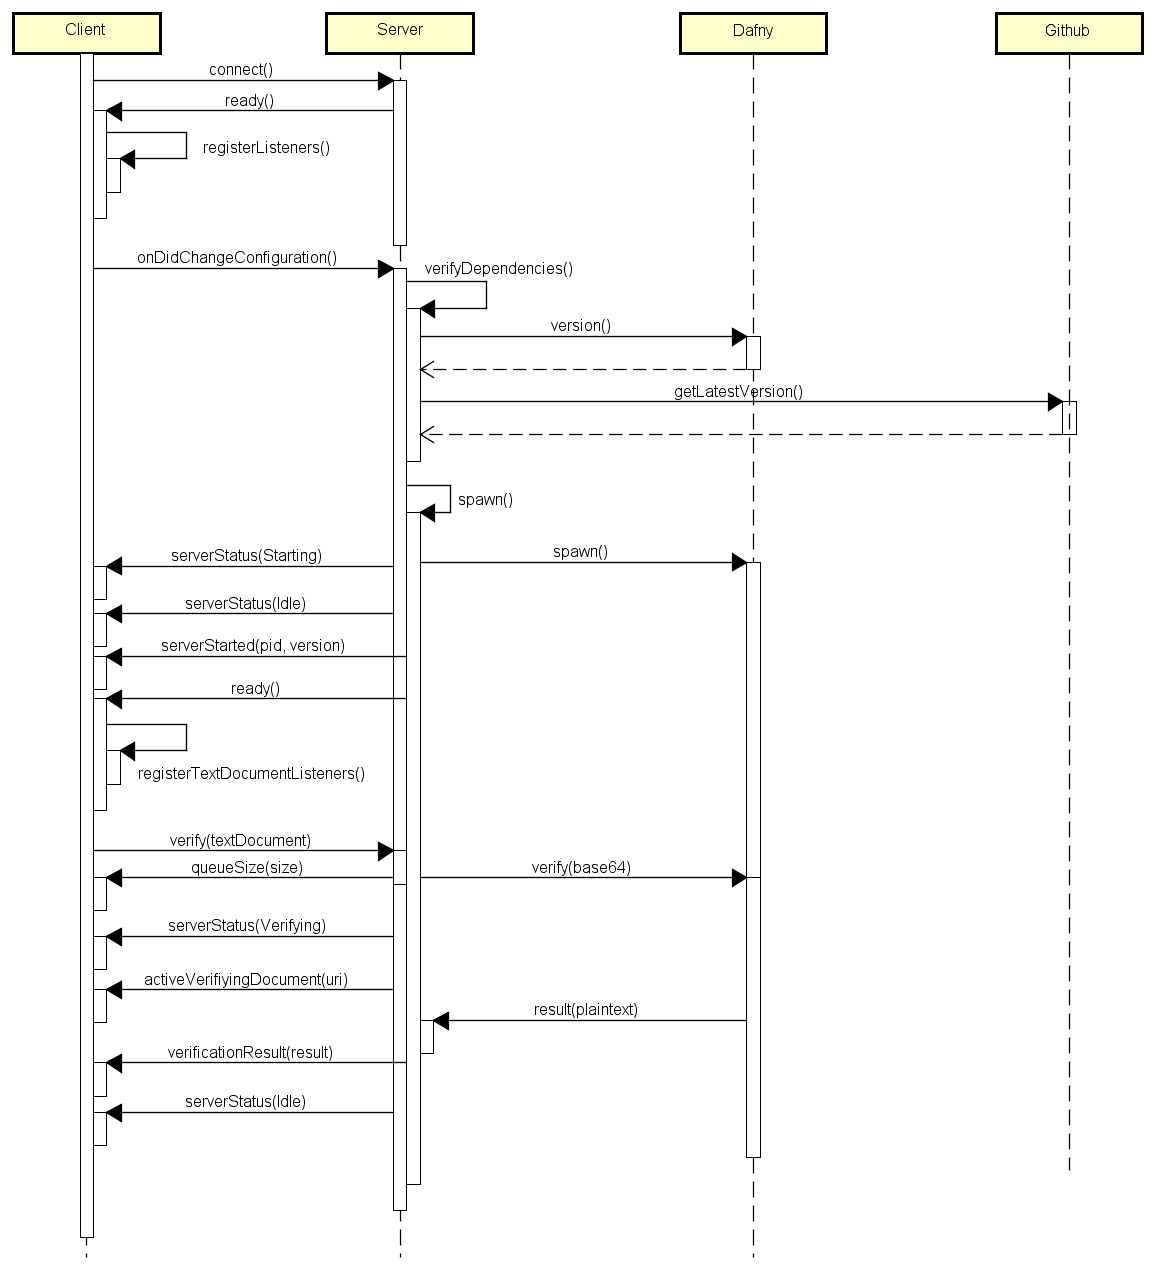
\includegraphics[width=1\textwidth]{img/DafnyStartupFull}
	\caption{DafnyServer startup}
	\label{fig:DafnyServer startup}
\end{figure}

\subsubsection{Not installed}
If Dafny is not installed, the user is informed that Dafny can not be started and asks if it should be installed. It either fails if the DafnyServer can not be started or the verb version is not implemented. If the answer is yes, the flow will continue in the next graphic on install()
\begin{figure}[H]
	\centering
	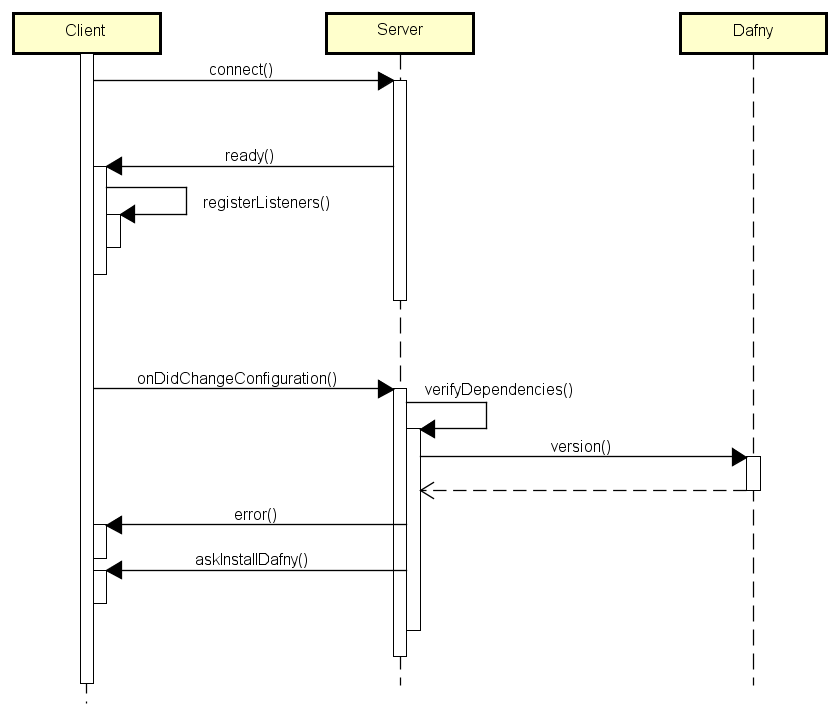
\includegraphics[width=1\textwidth]{img/DafnyNotInstalled}
	\caption{Dafny not installed}
	\label{fig:Dafny not installed}
\end{figure}

\subsubsection{Installation - Upgrade available}
After the version of Dafny is known and the comparison with the release information of GitHub shows that there is a newer release available. In that case the DafnyServer is started normally, but the user is also informed that there is a newer version. If the answer is yes, the installation starts. The first step is to stop the DafnyServer, if it is active, to perform after that an uninstallation regardless if Dafny was installed. Afterwards, depending of the platform, the correct release is downloaded from GitHub. During that step, progress notifications are sent to the client (not visible in the graphic). As soon as the download is finished the archive is extracted again with progress information. The last step is to do start over and do the verification again. 
\begin{figure}[H]
	\centering
	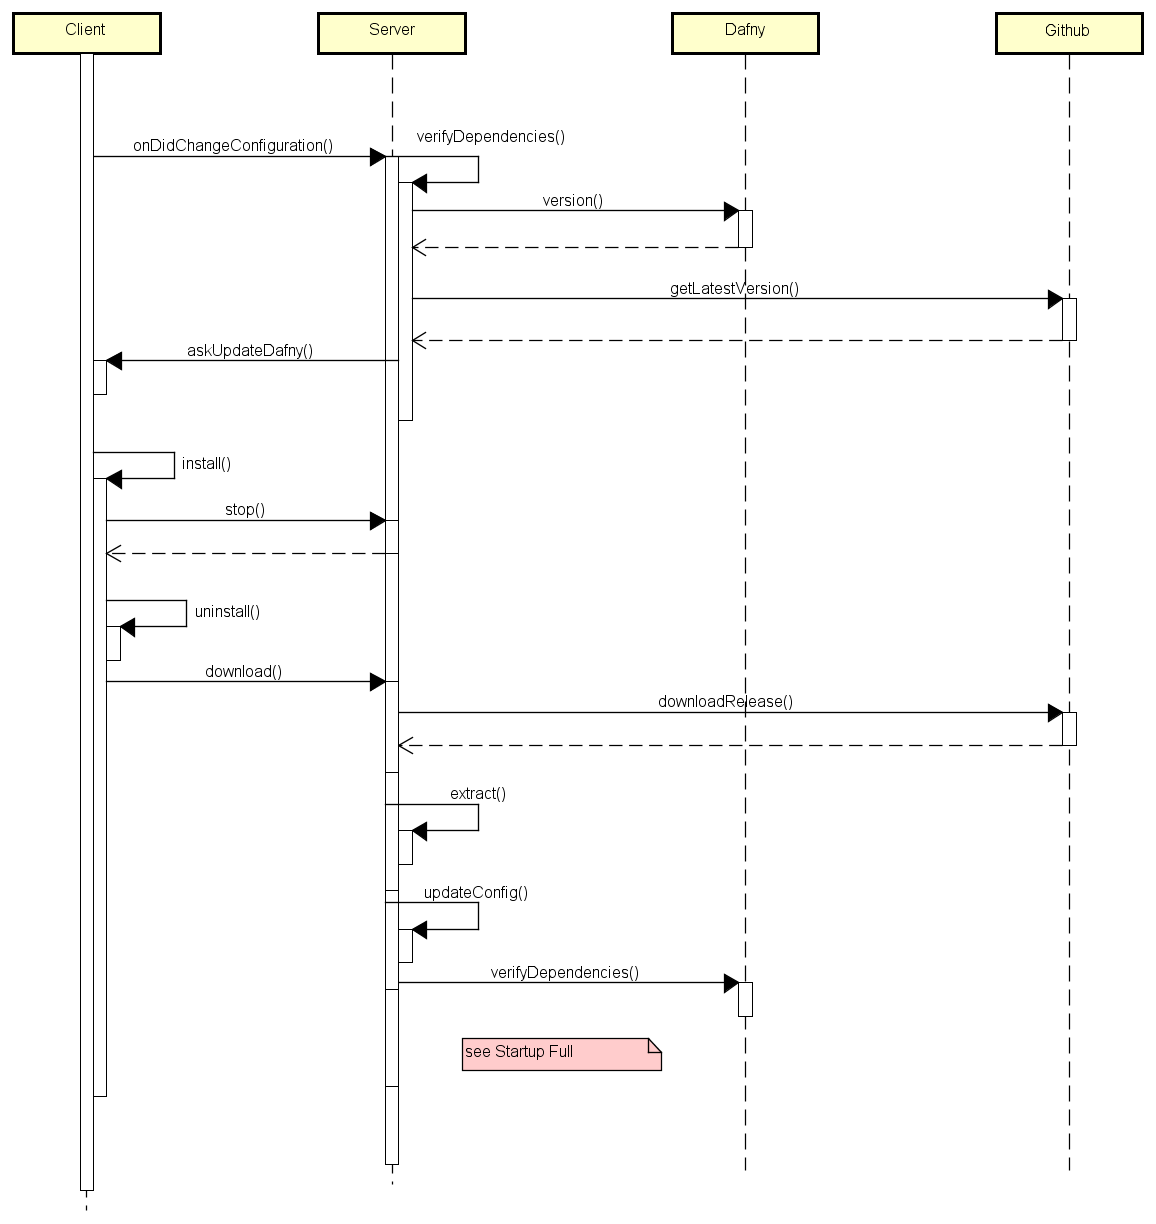
\includegraphics[width=1\textwidth]{img/DafnyVersionUpgrade}
	\caption{Version upgrade available}
	\label{fig:Version upgrade available}
\end{figure}





\subsection{Extension points}

\paragraph{Status bar}

\paragraph{Refactoring}

\paragraph{CodeLens}

\paragraph{Go to definition}

\paragraph{Debugger}
\todo{Boogie Verification Debugger: Why BVD can't be used directly: C sharp UI, }

\subsection{Communication}

\subsection{Syntax highlighting}

\subsection{Snippets}

\subsection{Automatic installation}
\subsubsection{Windows}

\subsubsection{Ubuntu}

\subsubsection{OSX}


\subsection{DafnyServer}
Github Repository: \href{https://github.com/FunctionalCorrectness/dafny-microsoft}{https://github.com/FunctionalCorrectness/dafny-microsoft}

The DafnyServer is a simple console application which allows proofing Dafny source files. To verify documents, they are sent over the standard input. Results are obtained from the standard output. The verification task needs to be in JSON format \todo{add reference to source.cs} and is sent base64 encoded. By default, the server only supports the verbs verify, quit and selftest. Verbs are sent first, followed by a newline \textbackslash{n}. They may be proceeded by a payload and an end string \textbf{[[DAFNY-CLIENT: EOM]]}. \newline 
Verb explanation: Verify needs a verification task and returns if all proofs holds, quit stops the server and selftest execute some simple verification. \newline

\textbf{Example verification task}
\begin{lstlisting}[language=json,firstnumber=1]
{
	args:[],
	filename:"c:\Users\Markus\Desktop\dafny\test1.dfy",
	source:"method Main() {	assert 1 < 3; }",
	sourceIsFile:false
}

\end{lstlisting}

\subsubsection{symbols}
To support refactoring in the Dafny Visual Studio Code plugin, symbol information was needed. All fields, methods and classes inside a file along with their information about position, reference and usage have to be accessible. To support this, the DafnyServer was extended. A new verb "symbols" was introduced. This collects various information about the symbol table of the input file and returns it as JSON. 
\newline\newline
\textbf{Request: }

\begin{lstlisting}[language=dafny]
class BankAccountUnsafe {
  var balance: int;
  constructor() modifies this { 
    balance := 10;
  }
  
  method withdraw(amount: int) 
    modifies this
    requires amount >= 0
  {   
    balance := balance - amount; 
  } 
}   

method test() { 
  var a := new BankAccountUnsafe(); 
  a.withdraw(9);  
}   
\end{lstlisting}

\textbf{Result: }
\begin{lstlisting}[language=json,firstnumber=1]
[ 
....
{
  "Call" : null,
  "Column" : 3,
  "EndColumn" : null,
  "EndLine" : null,
  "EndPosition" : null,
  "Ensures" : [],
  "Line" : 3,
  "Module" : "_module",
  "Name" : "_ctor",
  "ParentClass" : "BankAccountUnsafe",
  "Position" : 49,
  "References" : [{
    "Column" : 12,
    "Line" : 15,
    "MethodName" : "test",
    "Position" : 265,
    "ReferencedName" : "_ctor"
  }],
  "Requires" : [],
  "SymbolType" : "Method"
}, {
  "Call" : null,
  "Column" : 9,
  "EndColumn" : null,
  "EndLine" : null,
  "EndPosition" : null,
  "Ensures" : [],
  "Line" : 6,
  "Module" : "_module",
  "Name" : "withdraw",
  "ParentClass" : "BankAccountUnsafe",
  "Position" : 114,
  "References" : [{
    "Column" : 5,
    "Line" : 16,
    "MethodName" : "test",
    "Position" : 296,
    "ReferencedName" : "withdraw"
  }],
  "Requires" : ["amount >= 0"],
  "SymbolType" : "Method"
}, {
  "Call" : null,
  "Column" : 6,
  "EndColumn" : null,
  "EndLine" : null,
  "EndPosition" : null,
  "Ensures" : null,
  "Line" : 2,
  "Module" : "_module",
  "Name" : "balance",
  "ParentClass" : "BankAccountUnsafe",
  "Position" : 32,
  "References" : [{
    "Column" : 5,
    "Line" : 4,
    "MethodName" : "balance",
    "Position" : 85,
    "ReferencedName" : "balance"
  }, {
    "Column" : 3,
    "Line" : 10,
    "MethodName" : "balance",
    "Position" : 190,
    "ReferencedName" : "balance"
  }, {
    "Column" : 14,
    "Line" : 10,
    "MethodName" : "balance",
    "Position" : 201,
    "ReferencedName" : "balance"
  }],
  "Requires" : null,
  "SymbolType" : "Field"
}
.... 
]
\end{lstlisting}



\subsubsection{versioncheck}
To support automatic updates of the Dafny environment in a general approach, it was decided to implement this features directly into the DafnyServer. To make it as general as possible, the check is directly performed on release page of the Dafny project. The GitHub API allows to check this in just one call. Additionally, a semantic versioning library\cite{semver} was used to compare the current and the version from GitHub. Based on that, it either checks if an update is available or if the latest version is installed. If there is an update available, the URL to download the package can also be read out of the returned JSON 
\newline
\textbf{Response from GitHub}
\begin{lstlisting}[language=json,firstnumber=1]
[{
  "name" : "v1.9.12",
  "assets" : [{
    "name" : "dafny-1.9.12-x64-osx-10.11.6.zip",
    "browser_download_url" : "https://github.com/FunctionalCorrectness/dafny-microsoft/releases/download/v1.9.12/dafny-1.9.12-x64-osx-10.11.6.zip"
  }, {
    "name" : "dafny-1.9.12-x64-ubuntu-14.04.zip",
    "browser_download_url" : "https://github.com/FunctionalCorrectness/dafny-microsoft/releases/download/v1.9.12/dafny-1.9.12-x64-ubuntu-14.04.zip"
  }, {
    "name" : "dafny-1.9.12-x64-win.zip",
    "browser_download_url" : "https://github.com/FunctionalCorrectness/dafny-microsoft/releases/download/v1.9.12/dafny-1.9.12-x64-win.zip"
  }]
}]
\end{lstlisting}

Currently the check is performed against the URL:  \href{https://api.github.com/repos/FunctionalCorrectness/dafny-microsoft/releases}{https://api.github.com/repos/FunctionalCorrectness/dafny-microsoft/releases} which has to be changed as soon as the pull request is performed. 


\subsubsection{version}
The command returns the version of the DafnyServer.  


\subsection{Dafny}

\subsubsection{Unicode}
Dafny would support the following Unicode characters: 

\rowcolors{2}{gray!25}{white}
\begin{longtable}[H]
	{l|p{0.22\textwidth}| p{0.22\textwidth} | p{0.1\textwidth} | p{0.1\textwidth} | p{0.25\textwidth} | p{0.25\textwidth}}
	
	\textbf{Ascii} & \textbf{Unicode}  \\ \hline
	<==> & u21d4  \\  
	==> & u21d2  \\  
	<== & u21d0  \\  
	\&\& & u2227  \\  
	| | & u2228  \\  
	!= & u2260  \\  
	<= & u2264  \\  
	>= & u2265  \\  
	:: & u2022  \\  
	! & u00ac  \\  
	forall & u2200  \\  
	exists & u2203  
	
	
\end{longtable}

Unfortunately they are not working right know because of a bug in the parser.







\section{Architecture and Implementation} \label{architecture}
This chapter documents the architecture and the implementation of the plugin.

\subsection{Features} \label{features}
This chapter details the different features that were implemented during the project. They are mostly language agnostic features that were implemented according to the language server protocol to offer a richer IDE experience. The backbone of the language server protocol is the interface IConnection. When the plugin is started, an instance of this interface is established which allows communication from the client (the IDE) to the server (the plugin / the language server). On this connection, generic requests and replies can be sent and received, but the language server protocol also offers defined messages for common IDE features. Further insight into this can be won in \ref{langserver} \newline
For instance, if the plugin wants to support rename element, it must provide a callback to the onRenameRequest on the connection. The input to this callback usually is the information needed to answer the request, typically a document and a position in it. The language server is then free in its implementation on how to answer these requests. \newline
Usually this is done by a so called provider, a class which implements at least one method that can answer such a request. This method is then registered as a callback to that element when the plugin is initialized.\newline
This project also chose this approach, for every IDE feature a provider was implemented, which carries out the task of answering such a request. The providers themselves are heavily based on the symbol service. Both the providers and the symbol service are explained below.\newline 
\begin{figure}[H]
	\centering
	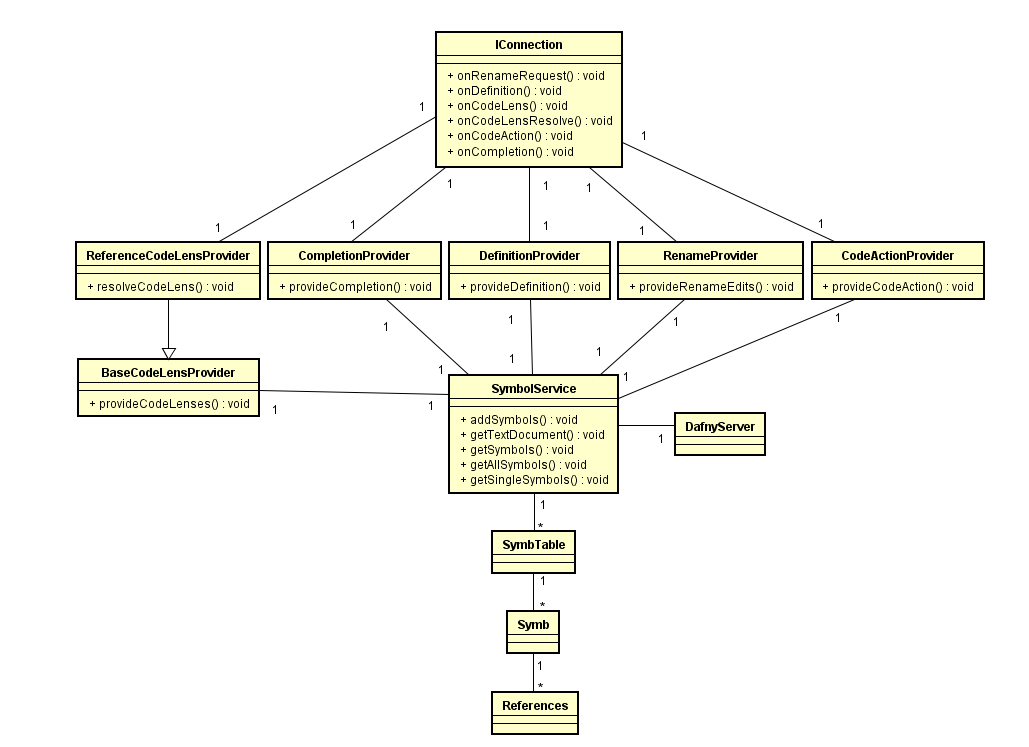
\includegraphics[width=1\textwidth]{img/featureArchitecture}
	\caption{How the IDE-features are integrated into the language server}
	\label{fig:featurearchitecture}
\end{figure}
\subsubsection{CodeLenses} \label{codelenses}
CodeLenses are Visual Studio Code a feature which is also common to many other IDEs. The idea is to display meta information about certain pieces of codes, for instance classes and methods. In Visual Studio Code this is done  by adding an additional line of text to the editor wherever a codeLense should  be placed. \newline
\begin{figure}[H]
	\centering
	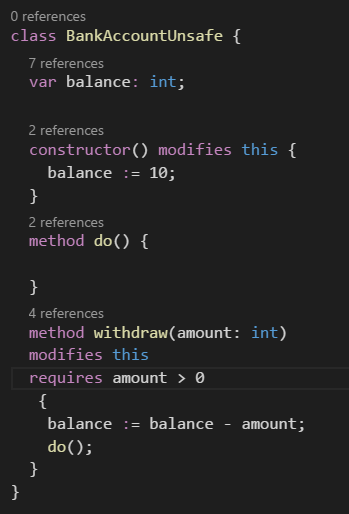
\includegraphics[width=0.5\textwidth]{img/codelensesClosed}
	\caption{Code Lenses used with Dafny}
	\label{fig:codelensesclosed}
\end{figure}
It was decided to display codeLenses for classes, methods (including constructors) and fields, since they tend to have a wide scope in the code bases \newline
A second consideration was which information should be displayed in a codeLens. When codeLenses are language specific and do not for instance stem from a plugin which displays code metrics or similar, usually references and usages of the element are displayed. It was decided to display this information also for the Dafny plugin. CodeLenses also allow commands to be executed when clicked upon, a logical conclusion is to implement go to reference when a reference in a codeLens is clicked.\newline
Since the tasks of finding the elements which need a codeLens and constructing the codelens itself are very different, the implementations were separated in a base class and a child class. The base class answers the onCodeLens request of the connection and the child class then answers the onCodeLensResolve request. The reasoning for this lies in possible future expansion, as maybe additional information should be displayed in a codeLens. This can be done in an own child class, the produced codeLenses (which stem from the same placeholder codeLens) then are automatically merged by Visual Studio Code. This design was also inspired by the GoLang Plugin \cite{godef}. 
\begin{figure}[H]
	\centering
	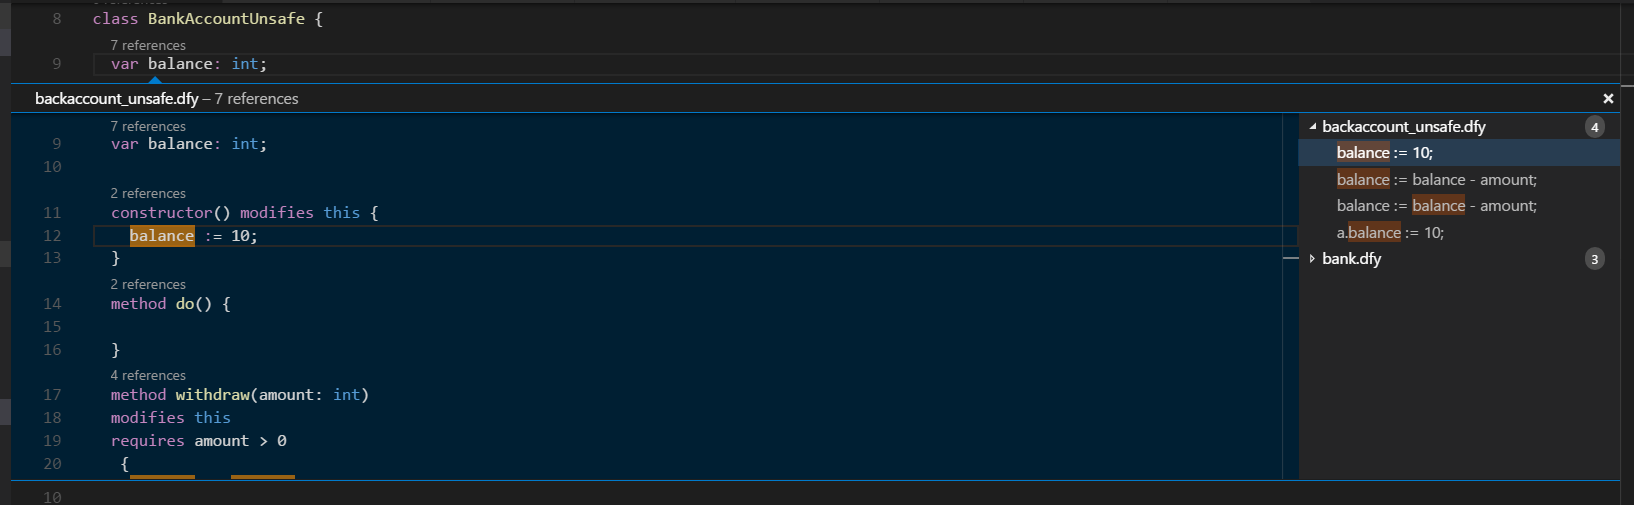
\includegraphics[width=1\textwidth]{img/codelensesExpanded}
	\caption{Expanded codeLens showing the references to the field balance}
	\label{fig:codelensesexpanded}
\end{figure}
The only challenging aspect when implementing this feature is that references can't be determined via a simple text search, since different classes could have members with the same name. To only display unambiguous references, the search has to be done via the fully qualified domain name of the symbol. Since information about references is needed often, all references are determined by the DafnyServer and returned together with the symbol information to the symbol service. This allows for simple processing in the language server itself and the references are updated in real time, since the symbol service refreshes the symbols for a file when it is changed. Off course also the file path belonging to the file in which the reference occurs is returned by the symbol service. This is needed when a reference is in  file external to the defining one and the go to reference command is invoked.\newline
When given locations of the references, it is possible to let Visual Studio Code highlight them in the preview window which opens when a codeLens is expanded. Visual Studio Code also groups references according to the file path in the location, so the programmer gets to see a map of all references ordered by containing file to the right of the preview window and can quickly navigate to them.
\subsubsection{Code Completion} \label{codecompletion}
Code completion has become a standard feature for IDEs. Usually, when the programmer starts typing, a little popup appears in which the programmer can choose options that complete the code he is currently writing. \newline
\begin{figure}[H]
	\centering
	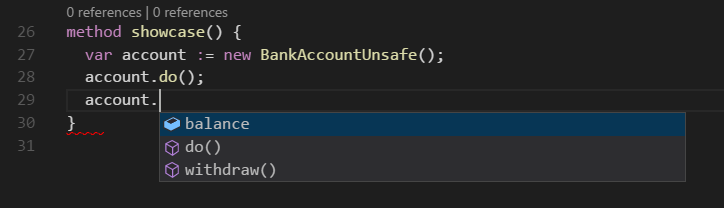
\includegraphics[width=1\textwidth]{img/codeCompletionOverview}
	\caption{Popup with completion options}
	\label{fig:codecompletionoverview}
\end{figure}
There are several different considerations when implementing code completion in a language server. The first one is to define which typed characters should trigger a completion request. Ideally, an IDE supports the programmer with completion regardless of the current context. Next to performance, another reason to narrow down the trigger selection is that not all contexts warrant meaningful suggestions for completion. In this project, a pragmatic approach was chosen where completion is triggered when ever a "." is typed, a situation where the programmer usually wants to access a member of an element. Since there is usually a designator present before the ".", there is also enough knowledge present about the current context to offer meaningful options. \newline
In order to support this, the symbol service stores all variable declarations so the plugin knows about the type of all expressions that can be followed by a ".". The completion request comes with a position in the current file as an argument, so the first task is to resolve the expression and find out the fully qualified name of each element. The language server then searches the symbol service for all members that are defined in the class with that fully qualified name and sends them back as completion suggestions. \newline
Visual Studio Code then handles all further actions, for instance, once the popup is displayed and the programmer continues to type, it removes all suggestions that don't start with the typed characters. It is also possible to display further information regarding the suggestions. The plugin already details if the completion is a field or a method, which Visual Studio Code provides  separate icons for. When the suggestion is a method, the preconditions, if any, are also displayed, so the programmer already knows the constraints he is writing under. \newline
 \begin{figure}[H]
	\centering
	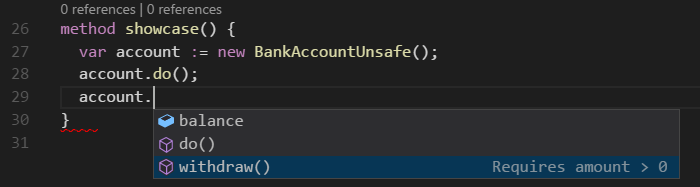
\includegraphics[width=1\textwidth]{img/codeCompletionMethod}
	\caption{Suggestion displaying precondition}
	\label{fig:codecompletionmethod}
\end{figure}
The implementation is straightforward, as the symbol service already provides ways to resolve the fully qualified name of an expression and if it as an alias for an element of a class, all therein defined methods and fields can simply be collected. The method and field symbols in the symbol services also contain all additional information which is displayed in the popup. Possible improvements in the completion feature would be support of built in methods and functions and also offer context aware completion when the programmer starts to type an identifier. 
\subsubsection{Go to Definition} \label{gotodefinition}
Another common feature is go to definition. It enables the programmer to quickly jump to the definition of a code element he is currently working with in order to gain further insight about it. This can usually be done either via a hot key for the current cursor position or an option when opening the context menu via a right click, Visual Studio Code offers both ways.\newline
\begin{figure}[H]
	\centering
	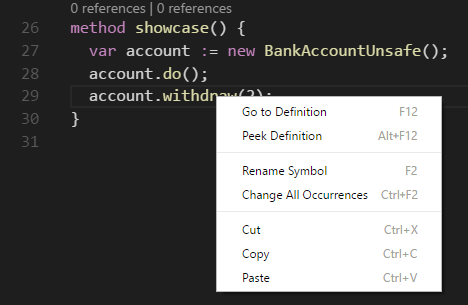
\includegraphics[width=0.5\textwidth]{img/goToDefinition}
	\caption{The Definition Features}
	\label{fig:gotodefinition}
\end{figure}
The language server protocol offers an on definition request, which has the URI of the file and the position for which a definition is requested as parameters. The plugin then first tries to resolve the word at the position which could lead to a definition. When a word could be resolved, the plugin tries to determine if the expression is an alias for an element of a class or if it stands for an access of a member of one. If this is the case, the fully qualified name of the symbol can be determined via the symbol service, as it stores information about all definitions and declarations. The plugin than finds the unambiguous definition via the fully qualified name and responds with the location of that definition. This also works if the definition is in an external file in the same workspace. \newline
If, for whatever reason, the fully qualified name cannot be determined, the plugin tries to match the selected word with any symbol cached in the symbol service. This approach only works as best effort though, as different classes could defines methods with the same name for example. If no match is found at all, no definition is provided. \newline
Visual Studio Code offers two options when searching for definitions, either go to definition which immediately opens the returned location in an editor or peek definition, which shows the definition in a little popup. \newline
 \begin{figure}[H]
	\centering
	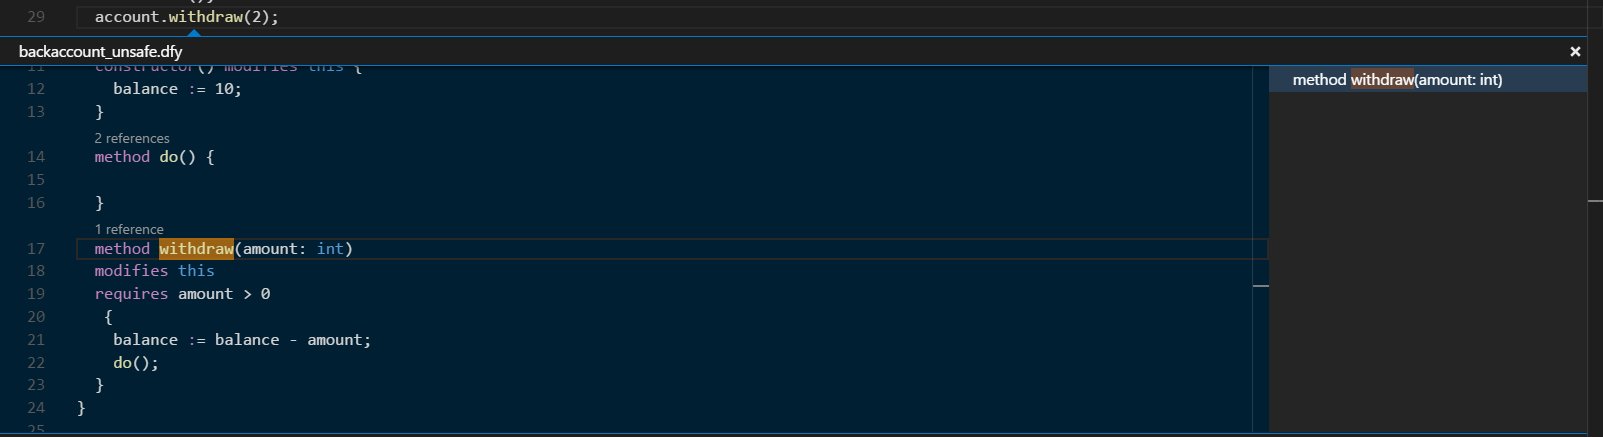
\includegraphics[width=1\textwidth]{img/goToDefinitionPeek}
	\caption{Overlay of peeked definition}
	\label{fig:gotodefinitionpeek}
\end{figure}
Extensions to this feature could be a context aware heuristic when a fully qualified name cannot be determined where for instance the current and nearby files are preferred when searching for definitions. Also, when polymorphism comes into play and the actual implementation cannot be determined, at the current state the first possibility is returned. The could be enhanced by offering all possible definitions.
\subsubsection{Rename Element} \label{renameelement}
Rename element is a feature essential to refactoring. It allows to quickly make code better readable. Visual Studio Code offers built in support for renaming either via a hot key or the context menu. \newline
The language server protocol, as with many other features, offers a request for renaming with the URI of the file in which the command was invoked and the position belonging to the command. Additionally, the new name of the element should have is also given as an argument. The protocol expects a collection of textedit commands, which entail an URI of file, and ranges in that file which should be replaced with a word. \newline
As often with the language server protocol, the first step when implementing the feature is to determine the element at the position which is given as an argument. When the position can be resolved to a meaningful word, the plugin tries to determine if it is either an alias for an element of a class, or a member of class, for instance a field or a method. If it can do so with absolutely certainty, the fully qualified name of that element is obtained. The next step is trivial, since the symbol service already caches all references to a symbol, information which it gained through the DafnyServer. The plugin can simply build textedits out of all references, since the reference already contain all necessary information such as the containing file and their position therein. This therefor also works across multiple files which reference the same element, as long they are open in the same workspace. Those textedits are then returned from the language server to Visual Studio Code, which does all the actual replacing. \newline
  \begin{figure}[H]
 	\centering
 	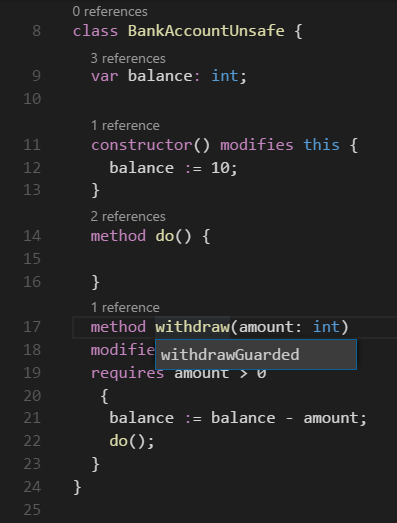
\includegraphics[width=0.5\textwidth]{img/rename}
 	\caption{Renaming an element in Visual Studio Code}
 	\label{fig:rename}
 \end{figure}
Since this feature actually changes code that is worked with, the implementation must be very robust and failsafe. Thus, it was implemented very defensive. It the location of a requested renaming cannot be resolved to a meaningful word, the request is ended without dictating any changes. The same holds if a word can resolved, but it cannot be matched to a fully qualified name. In this case, possible references could be ambiguous, so no action should be taken. To further limit the possibility for failure, the scope for this feature is very small. The current implementation only allows for renaming of class members such as fields and methods, since these can be resolved with absolute certainty.\newline
When extending this feature, it would be beneficial to also be able to rename local variables for instance. To do this, the symbol information which the DafnyServer returns to the symbol service would have to be enriched with detailed scope information to allow being able to exactly say which regions are prone to renamings and which are not. 
\subsubsection{Quick Fixes} \label{quickfixes}
Quick Fixes are a versatile feature in IDEs which basically allow to do any manipulation to code. Usually they are offered as reactions to diagnostics which were provided earlier. A simple example would be implementing a spell checker this way, offering to replace a wrongly written word with the correct spelling. \newline
Since this feature has no clear implementation guideline, and the plugin designer can implement almost anything that he likes this way, this was an obvious place to implement Dafny specific feature in the plugin.\newline
They way this works in Visual Studio Code is that when the diagnostic stage for the file has been completed, where all things such as compiler warnings or custom warnings are generated, a new request is fired at the language server. This request holds a collection of all diagnostics on the current file and the language server is free to either do nothing are provide commands for some diagnostics in the collection which often aim to resolve the shortcomings detailed by the diagnostic. \newline
  \begin{figure}[H]
	\centering
	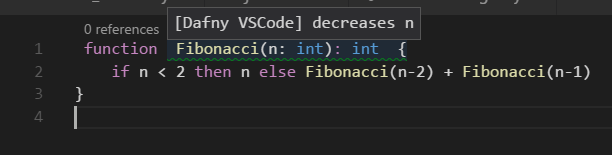
\includegraphics[width=0.7\textwidth]{img/diagnostic}
	\caption{Visual Studio Code displays a diagnostic}
	\label{fig:diagnostic}
\end{figure}
The current stand of the projects offers three code fixes to resolve Dafny specific diagnostics. \newline
The first one is a common situation where a programmer fails to capture his intention that an expression should either decrease or increase when working with recursion or loops. It can also be the case that an expression must always evaluate into a certain range, this is for instance the case when an expression that is used as an index to an array is not constant within a loop. The remedy is simple, a decrease / increase guard with the expression in question must be added at the correct location. In case an expression must be within a certain range, the same intent can be written as an invariant. \newline
  \begin{figure}[H]
	\centering
	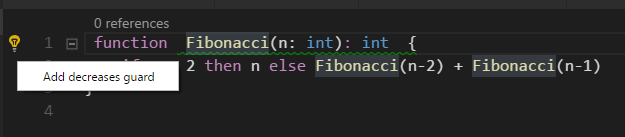
\includegraphics[width=0.7\textwidth]{img/decreaseGuard}
	\caption{Offering a code fix to add a guard}
	\label{fig:decreaseguard}
\end{figure}
This situation can easily be identified through the message within the diagnostic, since Dafny always gives this message in the same format. The expression that has to be decreased can also easily be parsed out of this message. The placement of the guard is a little more difficult, the implementation tries to find the first block in which the variables used in the expression are not in scope anymore. The guard is then inserted before the block containing the first usage. \newline
  \begin{figure}[H]
	\centering
	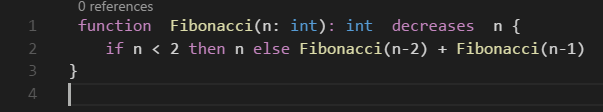
\includegraphics[width=0.7\textwidth]{img/decreaseGuardApplied}
	\caption{Program after the code fix}
	\label{fig:decreaseguardapplied}
\end{figure}
The second code fix the plugin offers is very similar, but this time the constraint is that an object may be null when it should not. The situation again is easily detected through the message in the diagnostic, and also the expression which should not be null can be parsed through it.
  \begin{figure}[H]
	\centering
	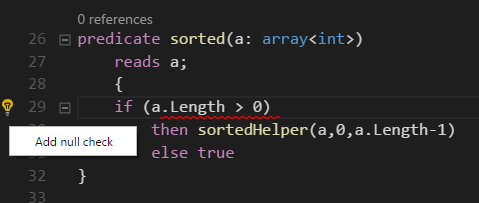
\includegraphics[width=0.7\textwidth]{img/nullCheck}
	\caption{It should be made sure that an element is not null}
	\label{fig:nullcheck}
\end{figure}
Also the search for the insertion position works very similarly. It then inserts the constraint in form of a precondition to the surrounding element. \newline
  \begin{figure}[H]
	\centering
	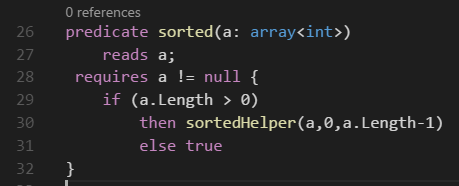
\includegraphics[width=0.7\textwidth]{img/nullCheckApplied}
	\caption{The precondition has been added}
	\label{fig:nullcheckapplied}
\end{figure}
The third code fix is to implement bound checking for expressions which are used to index an array. This can either take the form of a precondition, if the expression is constant within the block of code in question, are the form of an invariant if the expression is dynamic (for instance in a loop).
The remedy is to apply the bound checking either through preconditions or invariants, depending on the context.
  \begin{figure}[H]
	\centering
	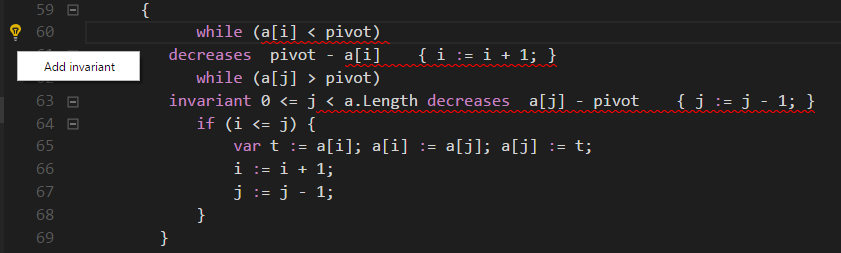
\includegraphics[width=1\textwidth]{img/indexOutRangeDiag}
	\caption{The expression may be out of range}
	\label{fig:indexOutOfRange}
\end{figure}
The first difficult part is to find the expression that is used as an index, as well as the identifier which stands for the array. Both is done through pattern matching on the code file in regard to the position of the diagnostic. Next it must be decided if preconditions or invariants should get generated, for this there must be knowledge about the context, e.g. if the expression is static in the current block. This is done via the information saved in the symbol service and also some pattern matching. \newline
Finally, the invariant or the preconditions must be inserted into the correct place. For this, all identifiers used in the expressions must be matched against their declaration, in order place the guards when already all symbols have been declared. \newline
  \begin{figure}[H]
	\centering
	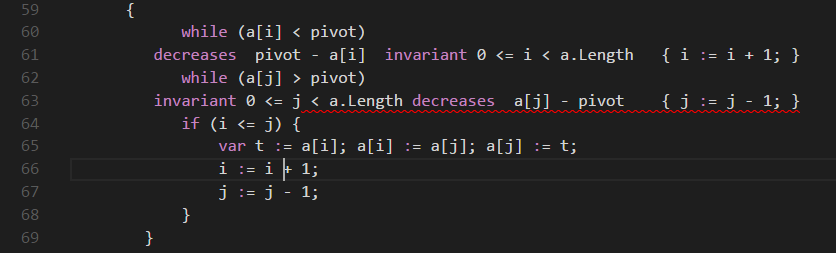
\includegraphics[width=1\textwidth]{img/indexChecked}
	\caption{Invariants for the loop were generated}
	\label{fig:indexInBound}
\end{figure}
At the current stand, only these three code fixes are implemented, the possible extensions are legion. One idea is to insert code that decreases a given expression when Dafny can't prove that an expression always decreases in a block were such a decrease clause was declared.\newline
\subsubsection{Counter Examples}
A useful features which also can provide a huge benefit, is to show an example which violates the contract, if the program can't be verified. Especially if the method is large with many branches, it can be very difficult to see how an example could look like which is not correct regarding the contract. \newline
Z3 verifies mathematical expression by trying to find a proof for the negation of the proof. That means if it finds a proof the program is not correct. But more important Z3 finds a assignment for the different variables which violate the contract. This knowledge can be used to show a counterexample in Visual Studio Code. The only big step is to translate the counterexample, which is called model in Z3, back into something that can be matched with the Dafny program. Fortunately this is already done in the DafnyProvider in Boogie. Additionally, to get only the necessary information out of it and also to show the values of class fields, the translation needed to be extended. A new server verb counterExample was introduced, which returns a counter example which is JSON encoded. Thereby it was possible to show assignments of the variables on each line in Visual Studio Code. \newline
This is a easy example of a invalid method which should return the ABS, but misses to handle negative numbers correctly. 
\begin{figure}[H]
	\centering
	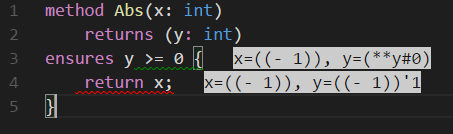
\includegraphics[width=0.7\textwidth]{img/counterModel}
	\caption{Counter Example is shown in Visual Studio Code}
	\label{fig:counterModel}
\end{figure}
Below is a more complex example of a class. The goal of the withdraw method is to prevent the balance to be below zero. Therefore the postcondition "ensures balance >= 0" exists. With help of the counter example it becomes clear that the amount is to big. It is bigger than zero though, but this precondition is wrong. It should be that the amount must be smaller than the balance. On the first line it shows that the balance is 2275 and the amount 2276 in the counter example. This results into the balance being negative after the subtraction. 
\begin{figure}[H]
	\centering
	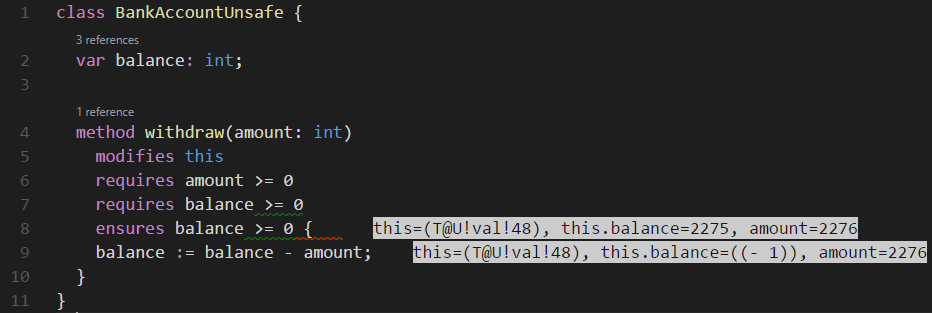
\includegraphics[width=1\textwidth]{img/counterModelBank}
	\caption{Counter Example inside a class}
	\label{fig:counterModelBank}
\end{figure}

\subsection{Environment}\label{environment}
This chapter details the underlying structure of the plugin which provides a basis to implement the individual concrete features.

\subsubsection{Symbol Service}\label{symbolservice}
The different features often need detailed information about symbols and their relations. A symbol table is a data structure used by a compiler to keep track of scope / binding information about names. These names are used in the source program to identify the various program elements, like variables, constants, procedures, and the labels of statements.\cite[239]{compiler} \newline
With regard to performance, but also to reduce overhead it was decided to implement a symbol service in the language server part of the plugin. It's main goal is to cache a subset of the symbol table of the compiler, such that features which need information about names in the code can use the symbol service to gain this insight without having to invoke the compiler every time a lookup has to be performed or each feature having to handle the information caching separately \newline
Since compilation is a heavy task, results should be cached efficiently. There is a trade off here though with the validity of the symbols, since if they are cashed too long, they don't represent the code anymore. The solution chosen is a lazy loading approach, meaning whenever a component queries the service the first time, the symbols are loaded and cached for the first time. This is usually done through by codeLenses, since they need the symbol information and they are created every time a file is opened right at the start. To make sure that no unnecessary loads are performed, the symbol table for each document is stored alongside a hash of the content of the document. Before sending a new request to DafnyServer, a comparison of the hashes is done to ascertain that the file really has changed. In future, this would also allow efficient caching by using histories of symbol tables when actions are undone. Next to the symbol table, it also stores the supplied text document itself, allowing for quick text manipulation if the content has not changed when loading the symbols.\newline
The next consideration was on how to store the symbol table and which information should be saved. The fields used are mostly needed to either determine which kind of symbol it is, where its scope is, its fully qualified name and relationships in form of references are also stored. This lead to the following data structure that is stored in the symbol service, the example is simplified for better readability: \newline
\newline\newline
\textbf{Symbol Tables: }
\begin{lstlisting}[language=json,firstnumber=1]
[
 {
  fileName: "filepathInUriFormat",
  hash: -483616355,
  symbols: [
   {
    call: null,
    column: 5,
    document: "filepathInUriFormat",
    end: Range(8, 12),
    ensures: [...],
    line: 8,
    module: "module",
    name: "balance",
    parentClass: "BankAccountUnsafe",
    position: 96,
    range(start, end),
    References: [
     {
      column: 4,
      document: "filepathInUriFormat",
      end: Range(11, 11),
      line: 11,
      methodName: "balance",
      position: 154,
      range: Range(start, end),
      referencedName: "balance"
     },
     ...
    ],
    requires: [...],
    start: Range(8, 5),
    symbolType: "Field"
   },
   ...
  ]
 },
 ...
]
\end{lstlisting}

The possible symbol types that are stored are defined as follows:
\begin{lstlisting}[language=json,firstnumber=1]
{
 Unknown,
 Class,
 Method,
 Function,
 Field,
 Call,
 Declaration	
}

\end{lstlisting}
The symbol table offers the following API to obtain symbols: \newline
\paragraph{addSymbols(doc: Textdocument, symbols: SymbolTable, forceAddition: boolean=false): void} This saves the supplied symbol table and associates it with the text document given. The default behavior is to get a new symbol table from the DafnyServer anyway and compare if they have changed. If so, the never one is chosen and persisted. If the parameter forceAddition is set to true, the symbol table is stored even though it might be out of date, a new version is not queried.

\paragraph{getTextDocument(uri: string): TextDocument} If the service has cached a text document specified by the Uri supplied, it returns it.

\paragraph{getSymbols(doc: TextDocument): Promise<SymbolTable[]>} Returns all the symbol tables that are stored in the symbol service. Optionally, a text document can be given as an argument. If the symbols to this document are not cached, then they are queried from the DafnyServer. Since this is an asynchronous operation, the return type is a promise of symbol tables. This method is useful when actions have to be done across the whole workspace.

\paragraph{getAllSymbols(doc: TextDocument): Promise<Symbol[]>} Similar to the method above, but the result is already flattened to an array of symbols across the whole code base. This is useful when it is not important to work with the symbols on a file per file basis.

\paragraph{getSingleSymbols(doc: TextDocument): Promise<SymbolTable>} This method allows for gaining the symbols for a single text document. If they are not cached yet, the service queries the Dafny Server for it, stores the result and then returns it. Since this operation is asynchronous, the return type is a promise.
\newline
When querying the the DafnyServer, the server defensively starts the communication with it by supplying the symbol verb, the file path and content for which it wants symbols on stdout. It then waits on the socket for a response, and if it is well formed and contains the queried symbols, the JSON returned by the server is parsed and the new symbol elements are constructed out of the JSON, which are then saved in the service. \newline
When there is an error, for instance a connection error, or there was a compilation error which prevents the building of a symbol table, the service deals with the error and just keeps, if it has any, the old symbol table of the file, so that the data is always in the most consistent state possible. Since compilation errors or connection errors are signaled to the user, the service listens until the broken elements have been repaired and then queries the server again for the symbols. \newline
Parsing of a successful response is also done conservatively, meaning that if an important property on for instance a method symbol is missing, this symbol is not stored, although all other valid symbols from that batch are stored. This allows for the maximum of analysis with only partly correct data. \newline
An improvement to the symbol service could be to do the caching more cleverly, for instance ignoring white space changes. A trade off in this area is that the calculations to decide if an update should be made could be more expensive then the update itself, so this should be monitored closely. Also when more and more complex refactoring and analysis should be done with the plugin, the data structure stored must probably be expanded. The extreme would be to save the whole AST in the symbol service which off course would be an overkill. Also here a balance thusly must be found between information richness and scope. Another consideration could be to optimize the lazy loading approach, for instance draw on a simple heuristic which files might be opened soon and load the symbols for them preemptively\newline



\section{Course of the project} \label{projectCourse}
This chapter details how the project was implemented and in what way it deviated of the project plan.

\section{Deviations from the project plan}\label{projectCourse}
This chapter details how the project was implemented and in what way it deviated of the project plan.
\subsection{UC3: Reporting of Dafny best practices violations}
While this idea seemed obvious when planning the project, this feature could sadly not be implemented. When working with different IDEs and well established programming languages, a programmer is often used to be supported by tools which can help write cleaner and more idiomatic code, such as linters. From this viewpoint, the integration of such a tool into the plugin seemed necessary. \newline
While established languages have a pool of agreed upon best practices, Dafny is still a very young language with not yet wide spread usage. The tooling around Dafny is also still not as sophisticated yet as for other languages. From this it can be inferred that there is not yet a big collection of programs to gain experience from, and that the problem of establishing a clear work flow with Dafny usually still exists, further preventing programmers to concentrate on idioms. \newline
These facts reflect why there is no collection of best practices for Dafny yet, either in form of some documentation or as a suggestion from people that are involved with Dafny. \newline
A second point worth noting in regard to this use case is how best practices for Dafny could look like. Dafny differs to most other languages in that it provides excellent specification constructs. A natural area to agree on idioms would therefor be the contracts of a piece of code. This could also greatly enhance the performance, because if clever usage is made of techniques such as short circuiting, a proof can be calculated at a much lesser cost than with a naive implementation. \newline
While providing support for best practices for contracts would therefor be very nice, this would also be almost unsolvable complex. Even for simple cases a deep understanding of proof theory would be needed, while for complex conditions it is not determinable if they can be proven in a better way or if they can be specified and proven at all. \newline
Since the establishment of own best practices for Dafny without being able to include an existing collection was deemed an unrealistic, and the structuring of contracts in the best way possible an unsolvable task, it was decided to concentrate on other features of the plugin instead. \newline


\subsection{UC4: Automatic generation of contracts}\label{missinguc4}
Since the biggest selling point of Dafny is the possibility to write specification constructs. It therefor was clear to try to provide automatic generation of some of such constructs in this project. While planning the project, the proof pipeline used by Dafny was not yet understood fully, the grasp on proof theory was quite small as well. This made it very hard to estimate if such a feature could be implemented at all and if so, in what time. Nevertheless the potential benefit of such a feature marked it as a milestone in this project. \newline
While researching the theoretical basis for implementing such a feature as detailed in \ref{examples} and the chapters following it, it became apparent that the topic was quite complex. A first stumbling block were invariants. As languages such as Eiffel \ref{eiffel} make it is to work with invariants, it was assumed that Dafny offers this possibility as well. \newline
As was learned, there are several different methodologies when it comes to invariants, having them implemented as a macro which simply inserts them as postconditions to every block is simply the easiest approach. A collection of techniques can be found in \cite{invariants}. 
Dafny doesn't build in object invariants because it doesn't commit to a particular methodology. Since the upholding of certain business rules (which was the aim of this use case) via specification constrains usually translates into generation of invariants, in addition to generating the invariants, it would have also been in the scope of this project to define how to deal with invariants in Dafny in a consistent work. It was also impossible to define and implement a way in which such business rules could be expressed regarding time and the trade off between usability and flexibility.\newline
The second idea was to apply the concept of the weakest precondition. This means that if a proof does not hold given a context, one can find the weakest precondition to make the proof valid. It would have been great to offer the generation of the weakest precondition as a refactoring in the plugin. However, since the weakest precondition must be expressed in Dafny, it would have to be found in almost human readable form. Z3 \cite{z3}, the theorem prover used by Dafny, tries to prove a theorem via contradiction, it is very hard to gain information about satisfiability from the prover. Additionally there is the problem that Dafny code gets translated to the Boogie\cite{boogie} meta language, which then gets translated to Z3 syntax. Even if one could gain information from Z3 about satisfiability, it would therefor be difficult to provide a matching back to the Dafny language and display this information. In general, the problem of inferring sufficient conditions for proofs is very hard if they should be human readable, the few existing solutions work with an iterative approach relying on stepwise reduction of counter example, for instance described in \cite{preInference}. This approach is difficult to implement and lacks the usability that was sought after in this use case.\newline
Lastly, it took a lot of time to gain a working knowledge of the proof pipeline. Since it consists of three big projects, namely Dafny, Boogie \cite{boogie} and Z3 working together, a deep understanding was not possible without having some existing knowledge in this time. While trying to understand the pipeline, it also became apparent that the knowledge of the authors in proof theory was not deep enough to really grasp the problem and work on a solution in a feasible time. \newline
Because of all these reasons, it was decided to not implement this use case in this project. While this is regrettable, other ideas were gained during the investigation of the problem. The feasibility of displaying counter modules was discovered, as well as small refactorings that provide constraints for a small, but very often needed set of instructions such as array accesses were thought of. The remaining time of this milestone therefor was directed at implementing these features instead. 

\subsection{Code Actions}\label{addCodeActions}
As detailed in \ref{missinguc4}, while trying to implement a proof of concept for contract generation, some often used concepts while working with contracts were discovered. This led to the idea to offer refactorings to generate the correct contracts for these concepts. While this is in no way a generic approach towards contract generation, it seemed as though these refactorings could help in many situations, making life considerably easier for the programmer. It was therefor decided to implement them, partly replacing the goals sought after in use case 4. A more complete picture, including an overview of the implementation, can be found in \ref{quickfixes}. The following list details on why these concepts were chosen. \newline
 
\paragraph{Null Check}
Programmers very often access members of elements, especially in the methodology of object oriented programming. While it offers a great way to structure a program and to represent reality in a program, it comes with some danger. The most common pitfall is what Hoare famously declared his biggest mistake\cite{hoare}, the null reference. To help avoid this, Dafny reports potential null reference. Since almost any piece of complex code deals with objects, this is a very common occurrence, since for instance every object given as an argument must be checked for null first. \newline
It was decided to offer a mitigation of this important, but tedious work. The plugin detects warnings about potential null references, and offers to generate a precondition that demands that the designator standing for the potential null reference may not be null. If the programmer accepts the proposal, the precondition is inserted at the correct location. This shifts the burden of providing a valid context to the caller of the method, so the method can concentrate on offering a solution to the call. While working with Dafny, it was noticed that such a precondition was needed for about every third method, meaning that a lot of work is done for the programmer by supplying this precondition generation.
\paragraph{Bound Checking}
Almost as often as checking for null, it is necessary to check if an index to an array is in bound. Dafny already has sufficient knowledge about the array data structure that it issues a warning every time it is not clear if an index that is used to access an element is in bound of the array. While programming with Dafny, it was observed that this is the case in almost every non trivial example using arrays. Since the array data structure is used quite often in Dafny, it was decided to also help the programmer with this construct, since bound checking is important, but tedious. \newline
Whenever a warning is issued by Dafny that an index may be out of bound, the plugin offers to generate two preconditions, namely one that states that the expression representing the index must be bigger than zero, and one that states it must be smaller then the array length minus one. The placement off course must be so that the preconditions are introduced at a place in the program where all variables used in the expression have been declared. When the programmer decides to use the quick fix, the preconditions are inserted and relieve him of the hassle of manually checking the bounds of the index.
\paragraph{Increase / Decrease / Invariant Guards}
Another concept that often arises when using Dafny is to make sure an expression converges to a certain range of values over time. This is the case when making use of recursion to ensure that the base case is eventually met, or when writing loops that depend on a certain value of an expression for termination. Both examples are very important, because not handling them correctly can result in endless loops or overflow. Dafny already does a good job in generating warnings that tell the programmer that constraints should be enforced for a certain expression. \newline
These situations also occur very often, since both recursion and loops are fundamental elements of programming, it was decided that the generation of these constraints could greatly benefit the programmer. In order to do this, the plugin offers to add an increase / decrease clause with the correct expression in place when Dafny detects recursion or a loop. When the programmer chooses to use the quick fix, the guard statements are inserted at the correct place. Another important constraint when working with loops goes hand in hand with the use case described above, namely when an array is accessed within a loop and the expression used as an index is not constant within the context of the loop. For this, Dafny offers the construct of invariants, that ensure that an expression is within a certain range during a given context. The plugin therefor offers to generate invariants which ensure that an expression used as an index is always in bound of the array. When the programmer chooses to use this feature, the invariant is inserted at the correct context. 

\subsection{Counter Examples}
A concept which was not known as the project started, were counter examples. They provide a huge benefit, as to understand how a program violates its contract. Especially if it is a more complex software with many methods and many branches, it can be very difficult to understand why a contract does not hold\newline
For this reason it was decided to implement that feature in addition to CodeActions \ref{addCodeActions}. 
Developers can use this practical features directly in Visual Studio Code. It shows on each line how the variables have to be assigned that the proof fail. \newline
Because the calculation of the model, how it is called in Z3, can take very long, it is not calculated automatically if a proof fails. Nevertheless this can be overridden in the configuration. 

 
\subsection{Displaying Flow Graph}
Something which is already implemented in Boogie, is the generation of a Flow Graph out of a boogie program. Because this could be quite useful for developers, it was decided to implement this feature as well. Mainly because it can be implemented so, that on one side is the source code and next to it, the flow graph. It displays the program visually including all pre- and postconditions. 


\section{Possible points for Extension} \label{extensions}
This chapter details what further work could be done on the plugin by subsequent projects.

\subsection{Support for other IDEs} \label{ides}
Since the plugin is structured as a language server, it should theoretically be possible to integrate it into any IDE which implements the language server protocol without any problems. In reality, some customization is often needed and some popular IDEs also do not fully implement the protocol yet. This chapter details which IDEs were looked at as possible hosts for the plugin and what would have to be done for a complete integration.

\subsubsection{Eclipse integration}
The eclipse project \href{https://projects.eclipse.org/projects/technology.lsp4e}{LSP4E} aims to integrate existing language servers into the Eclipse IDE in a easy way. 
\newline
"It includes some APIs to turn language server protocol elements into Eclipse IDE concepts and a generic integration allowing to easily plug any language server to an Eclipse IDE instance without need to write Java code, either via a plugin associating a new language server, and by letting users manually bind language servers to their IDE." \cite{lsp4e}

It is built on top of \href{https://github.com/eclipse/lsp4j}{LSP4J}, a Java implementation of the language server protocol. 
\newline
Integrating the Visual Studio Code Dafny language server into Eclipse could become possible in the future. Right know there is no way to interact on the client side as well. One only can specify a language server based on a program (NodeJS) and arguments (extension.js) which is executed and used for querying information. One can't add any behavior to Eclipse itself, which would be necessary for certain features. Also, the sendRequest isn't implemented yet (Commit: 1615e07), which is important for starting the DafnyServer correctly. 
The better way would be to program a new Eclipse plugin, based on LSP4J, which then would also allow to customize the status bar, run scripts and show progress information. 


\subsubsection{Emacs integration}

Emacs \cite{GNU} is a versatile IDE which enjoys great popularity especially in the open source community. Written in LISP, Emacs traditionally supported language integration via so called modes, which are demons that run in the background. This is already a similar architecture as used in a language server integration. \newline
Work on integrating languages servers into Emacs has already be done. The project emacs-lsp \cite{emacsLsp} aims to provide the connection between Emacs and language server. The project itself is structured as a classical Emacs demon and allows interactions with language server. There already exist some integrable language servers in languages such as Java or Haskell. The integration of emacs-lsp and existing language servers seems to be pretty trivial, an example can be seen in \cite{javaEmacs} using Java. \newline
Since the language server allows custom messages to be defined as detailed in \ref{langServer}, the Dafny plugin defines some of them. One set of custom messages is necessary since the plugin allows for downloading the Dafny compiler automatically and the communication in regard to this feature must be extended to the IDE, so that the user is aware of this feature. Additional custom components are the state of the file so that the programmer sees if it is verified or not, or the displacement of counter examples for proofs.\newline
These features were deemed very useful in this project, such that they should be a part of every IDE integration. This means that a little wrapper would have to be written on the client side of the language server which understands the custom messages and can relay this information to the IDE itself. The work that has to be done is trivial, since it simply means to pass information on and display them accordingly. \newline
It was decided that gaining a working knowledge of LISP and Emacs in order to write such a wrapper was not in the scope of this project. For a programmer familiar with Emacs and LISP this task should take no more than a week. The custom messages that need to be implemented can be found in  \ref{langServer}. It can be argued that this extensions should be one of the first ones to be tackled by later work, as one can gain a considerably larger user base without having to invest too much work. \newline

\subsubsection{Monaco Editor}
Monaco\cite{monaco} is the code editor that powers Visual Studio Code. It is also possible to use Monaco as a standalone editor in the browser. It would be intriguing to integrate Dafny directly into Monaco, since there aren't many simpler setups imaginable as simple opening a browser window. It was therefor decided to look into a possible integration of the plugin during the course of this project. \newline
 It soon became apparent that the project does not seem very active, as the latest commit was two months old at the time of this writing. The documentation for developers is also very sparse. Since the plugin is structured as a language server, there was hope that an integration would be trivial. However, Monaco does not implement the language server protocol. In the documentation, it can even be read that "Extensions written for Visual Studio Code will not run in Monaco"\cite{monaco}, without any further explanation given. \newline
 However, integrating a new language into Monaco is possible, as can be seen in an example for Typescript in  \cite{monacoType}. However, the setup is different than a language server integration or a Visual Studio Code plugin, it is questionable how much code could be shared. While the idea of running Dafny in an editor in the browser is interesting, the work that would have to be done in order to achieve this was deemed to be outside of the scope of this project. Additionally, if further work aims to implement this integration, an evaluation on how active the work on Monaco is should be done first, given the apparent standstill in the project at the time of this writing.\newline
\subsection{New Features} \label{featureExtensions}
This section details some interesting ideas that were gathered during development of the plugin, but were sadly out of scope of this project. It is thought as a starting point for developers that want to extend this plugin. 
\subsubsection{Debugger}
Integrating a debugger into the plugin would be great, since this is a feature that is very often used and very helpful when searching for bugs. An existing solution already support this feature, namely the Visual Studio integration \cite{visualstudiodafny} of Dafny. This already works very well and can be used as a guideline when developing an own integration. It is also a feature that programmers have become used to in all modern IDEs so it should be part of any language integration. \newline
Sadly it is also quite a difficult task since the interaction between an IDE, an executable and a debugger is complex. While the Visual Studio integration is open source, it is written in C\# and can therefore interface directly with the Dafny pipeline, which is heavily done in that integration. It would take quite some work to abstract this direct interaction into a clean API that extends the existing API of the Dafny pipeline. Using this API, a language server could provide an own implementation of a debugger.\newline
Designing this complex component was well out of scope for this project. It is estimated that, depending on the preexisting knowledge, this would be an endeavor of about two to four weeks time and probably would have to rely on at least some help by the Dafny development team. While this task is difficult, the result would be having an important feature that all users of modern IDEs anticipate in a language integration. It therefore should be a primary consideration when deciding on how to extend this project. 
\subsubsection{Widening Scope}
While many features have been implemented during the course of this project, the scope of their application was often narrowed as to provide a pragmatic approach to the problems regarding the scope of the project. For example, the rename element refactoring only works on members of classes, but not on parameters of methods. \newline
The exact scope of all features can be found in the API documentation of this project. While the extension of scope of existing features might seem tedious and not very interesting, it can introduce subtle problems that have to be dealt with with great care. It also is benefical to the users, as they can apply features in much wider contexts. 
\subsubsection{Contract Generation}
While contract generation has been implemented for some often occurring situations as detailed in \ref{dffeatures}, there is still a big potential for improvement in this area. Since a generic approach to contract generation has been deemed to be unfeasible, the next best way is to offer help in writing specification constructs in specific situations.\newline
When deciding to do work in this area, it is important to first analyze which situations appear often in a typical Dafny program. While this task it is difficult in itself, since it requires some expertise in Dafny, it is important because otherwise features may be implemented that do not get used in every day scenarios. \newline
When such situations have been identified, the specification construct generation must absolutely be correct. Since this is a feature that changes existing code, it is better to not provide any help when there is ambiguity regarding the correct solution. However, when done correctly, this is a feature from which programmers can greatly benefit, since it enhances productivity by eliminating the need to do complicated reasoning. It also introduces capabilities of Dafny to programmers that are not yet proficient in their usage of the language.



%\section{Ergebnisse}
[Placeholder]
%\section{Ausblick}
[Placeholder]

\appendix

\listoffigures
\addcontentsline{toc}{section}{\listfigurename}

\listoftables
\addcontentsline{toc}{section}{\listtablename}
\printbibliography[heading=bibintoc]
%\section{Anhang}
[Placeholder]
\end{document}
